% PLEASE USE THIS FILE AS A TEMPLATE
% Check file iosart2x.tex for more examples

% add. options: [seceqn,secthm,crcready]
\documentclass[sw]{iosart2x}
%\usepackage{dcolumn}

\usepackage{graphicx}
\usepackage{listings}
\usepackage{xcolor}
% \usepackage{caption}  % To use \captionof outside of floats

\definecolor{keywordcolor}{RGB}{255,127,0} % Custom color for keywords
\definecolor{lightgray}{rgb}{0.95, 0.95, 0.95} % Define a very light gray color

\lstset{
    language=Python,
    basicstyle=\ttfamily\scriptsize, % Smaller font size
    keywordstyle=\color{keywordcolor}\bfseries,
    commentstyle=\color{gray},
    stringstyle=\color{blue},
    showstringspaces=false,
    frame=single,
    breaklines=true,
    tabsize=4,
    numbers=left, % Disable line numbers in the margin
    backgroundcolor=\color{lightgray}, % Light gray background color
}

%%%%%%%%%%% Put your definitions here

%%%%%%%%%%% End of definitions


\pubyear{0000}
\volume{0}
\firstpage{1}
\lastpage{1}

\begin{document}

\begin{frontmatter}

%\pretitle{}
\title{Knowledge graph usage metadata: Insights from SPARQL log analysis
}
\runtitle{Knowledge graph usage metadata: Insights from SPARQL log analysis}
%\subtitle{}

% For one author:
%\author{\inits{N.}\fnms{Name1} \snm{Surname1}\ead[label=e1]{first@somewhere.com}}
%\address{Department first, \orgname{University or Company name},
%Abbreviate US states, \cny{Country}\printead[presep={\\}]{e1}}

% Two or more authors:
\begin{aug}
\author[A,B]{\inits{M.}\fnms{Maryam} \snm{Mohammadi}\ead[label=e1]{m.mohammadi@maastrichtuniversity.nl}%
\thanks{Corresponding author. \printead{e1}.}}

\author[A,B]{\inits{Ch.}\fnms{Chang} \snm{sun}\ead[label=e2]{chang.sun@maastrichtuniversity.nl}}

\author[A,B]{\inits{R.}\fnms{Remzi} \snm{Celebi}\ead[label=e3]{remzi.celebi@maastrichtuniversity.nl}}

\author[A,B,C]{\inits{ch.}\fnms{Christopher} \snm{Brewster}\ead[label=e4]{christopher.brewster@maastrichtuniversity.nl}}

\author[A,B]{\inits{M.}\fnms{Michel} \snm{Dumontier}\ead[label=e5]{michel.dumontier@maastrichtuniversity.nl}}

\address[A]{Institute of Data Science, Faculty of Science and Engineering, \orgname{Maastricht University}, \cny{The Netherlands}}
\address[B]{Department of Advanced Computing Sciences, Faculty of Science and Engineering, \orgname{Maastricht University}, \cny{The Netherlands}}

% \printead[presep={\\}]{e1,e2,e3,e4,e5}
% \address[]{\orgname{Institute of Data Science}, Maastricht University, Maastricht, 6229 EN \cny{The~Netherlands}}
\address[C]{Data Science Group,\orgname{TNO}, Soesterberg, \cny{The Netherlands}}

\end{aug}

%\begin{review}{editor}
%\reviewer{\fnms{First} \snm{Editor}\address{\orgname{University or Company name}, \cny{Country}}}
%\reviewer{\fnms{Second} \snm{Editor}\address{\orgname{First University or Company name}, \cny{Country}
%    and \orgname{Second University or Company name}, \cny{Country}}}
%\end{review}
%\begin{review}{solicited}
%\reviewer{\fnms{First} \snm{Solicited reviewer}\address{\orgname{University or Company name}, \cny{Country}}}
%\reviewer{\snm{anonymous reviewer}}
%\end{review}
%\begin{review}{open}
%\reviewer{\fnms{First} \snm{Open Reviewer}\address{\orgname{University or Company name}, \cny{Country}}}
%\end{review}

\begin{abstract}
Knowledge Graphs (KGs) are key technologies that enable enhanced understanding, knowledge representation, reasoning, and interpretation of complex data. The use of RDF KGs relies heavily on SPARQL queries for knowledge retrieval and manipulation. Analyzing SPARQL query logs can provide valuable insights into KG usage, revealing patterns in user behavior and interactions with the data. Prior studies have analyzed these logs in terms of their syntax and structure, but little is known about what parts of a KG are queried by users. This paper introduces content-based methods for analyzing KG usage, specifically examining the extent to which SPARQL queries cover the KG schema over defined time periods. We examine organic and robotic queries of Wikidata and Bio2RDF. Raw schema coverage is higher for robotic queries (60--97\%) than organic ones (14--21\%), but because the two query types differ greatly in volume, we control for sampling effort using individual-based rarefaction. This reveals a KG-dependent picture: on the compact, specialized Bio2RDF the broader robotic coverage is a genuine behavioral difference (robotic exercises $\sim$1.8$\times$ more of the schema at equal effort), whereas on the very large Wikidata the gap is largely a sampling-size artifact. Both datasets exhibit a sharp decline in usage frequency, indicating that a large set of schema elements is only infrequently queried. We perform statistical assessments to discover the trends and shifts in schema element usage across different KG versions, query types, and log intervals. Our work sheds light on KG usage, highlights frequently used schema elements as well as underused elements, and provides guidance for improvements in documentation, schema design, and performance optimization.
\end{abstract}

\begin{keyword}
\kwd{Usage Metadata}
\kwd{RDF Knowledge Graph}
\kwd{SPARQL Query Logs}
\end{keyword}

\end{frontmatter}

%%%%%%%%%%% The article body starts:

\section{ Introduction }\label{s1}

Knowledge Graphs (KGs) are widely used as they are powerful representations of complex data. By organizing data into graph structures and ontologies, KGs facilitate semantic data integration, advanced search capabilities, and building neuro-symbolic  models \cite{abu2021domain,peng2023knowledge}. The Resource Description Framework (RDF) is a common model to implement a semantic KG. RDF KGs represent data as triples (subject-predicate-object), which allows for flexible and machine-readable descriptions of entities and their relationships. This standardized format is widely used for Linked Data on the Web \cite{ali2022survey}. SPARQL endpoints enable programmatic interaction with RDF KGs using the SPARQL language, and these interactions can be stored in a web server.  Analyzing the SPARQL query logs offers insight into what users are interested in and the manner in which they access desired information \cite{bielefeldt2018practical}, revealing patterns in computational demands, reliability, performance, user behavior, and data modeling decisions \cite{asprino2023your, mohammadi2022semi, Handschuh2010LearningFL,bonifati2017analytical,kaminski2018complexity, picalausa2011real,lorey2013detecting, raghuveer2012characterizing,rietveld2014man}. 

Throughout this paper we use three terms consistently. A \emph{type} (or class) is a resource used to classify instances, i.e., the object of a typing predicate such as \texttt{rdf:type}/\texttt{wdt:P31} or a subclass predicate such as \texttt{rdfs:subClassOf}/\texttt{wdt:P279}. A \emph{predicate} is the property in a triple $(s,p,o)$. An \emph{individual} is an instance, i.e., a non-schema resource (for example, a specific drug or person). We refer to the set of distinct types and predicates of a KG as its \emph{schema elements}.

Previous studies on SPARQL query logs have primarily focused on the syntax and structure of these queries. These studies have analyzed keyword usage (e.g., count of SELECT, ASK, UNION, OPTIONAL) and query shapes (e.g., chain, tree, cycle), and their relation to evaluation complexity \cite{bonifati2020analytical, buil2015preliminary, saleem2015lsq,stadler2024lsq}. More recent work has begun to examine \emph{which} schema elements are queried: Bonifati et al. \cite{bonifati2019navigating} analyze predicate usage in Wikidata query logs (including an interactive property sunburst), and Hammerer and Martens \cite{hammerer2025compendium} catalog the Wikidata IRIs used for transitive (property-path) navigation. Asprino et al. \cite{asprino2023your} employed a content-centric approach to summarize query logs and identified query templates that qualitatively characterize user queries, revealing patterns and contexts in which different types, relations, and instances are used. What is still missing, and what we provide, is a \emph{quantification} of how much of a KG's schema is covered by queries, of the usage frequency of each schema element, and of how this coverage shifts over time and between organic and robotic query types across two contrasting KGs.
This study explores ways to better understand the usage of KGs through the analysis of SPARQL query logs. We present novel methods to quantify schema (types and relations) usage, as well as to measure the frequency and the extent of that usage. Our research seeks to answer two main questions: (1) How can we quantify the usage of a KG? and (2) Do frequency distribution and ranking analyses of used KG elements reveal usage patterns over different log intervals or across organic (human-driven) and robotic (bot-driven) query types?

Previous work \cite{mohammadi2024analyzing} reported that most of the schema (types and relations) of the Bio2RDF KG was referred to within the SPARQL query logs over 30 months of queries. However, this work provided only a superficial view of user interaction with the KG, lacking deeper insights into the extent to which each schema element is accessed by users as well as differentiating between human and robotic interactions. 

In this study, we extend prior work \cite{mohammadi2024analyzing} to scrutinize the extent to which each schema element is included in user SPARQL queries while differentiating between organic and robotic queries from two KGs: Bio2RDF and Wikidata. The output of this analysis can be termed "usage metadata". The method produces novel usage metadata that offers practical insight into the extent to which KG is used by SPARQL users. Such information may be useful in understanding what users are querying in the KG and for targeted optimizations toward enhanced user engagement and operational efficiency. 
An innovative aspect of our approach is that it focuses on the triple patterns in SPARQL queries so as to focus on the types, relations, and individuals referred to in the queries. The main contributions of this paper, relative to preliminary work \cite{mohammadi2024analyzing}, are as follows:

\begin{itemize}
\item \textbf{A robust pipeline for recovering schema elements from raw query logs.} Raw logged query strings are frequently unparseable (missing prefix declarations, URL-encoding, appended HTTP parameters). We describe a preprocessing pipeline (prefix injection, URL-decoding, parameter removal, placeholder substitution, and variable standardization) that makes the logged queries parseable and aligns the schema extracted from the query side with the schema extracted from the KG side over a consistent reference set of subgraphs (Sections~\ref{s3}.3--\ref{s3}.4).

\item \textbf{Identification and analysis of usage patterns in query logs.} We compute schema-element frequency distributions and conduct statistical assessments (Shapiro--Wilk, Wilcoxon signed-rank, Spearman's rank correlation) to evaluate the consistency of, and changes in, schema-element usage in both Wikidata and Bio2RDF across KG versions, query types, and log intervals.

\item \textbf{A size-controlled comparison of organic vs.\ robotic coverage.} Because logs of different query types differ greatly in size, raw coverage differences can be sampling-size artifacts. We add an individual-based rarefaction analysis (and Chao1 richness estimation) that compares schema coverage at equal sampling effort, disentangling genuine behavioral differences from differences in query volume.

\item \textbf{Demonstrated applicability to additional logs.} We apply the methods to new intervals of Bio2RDF and Wikidata logs across two KGs of very different scale and style.
\end{itemize}
The organic/robotic distinction itself is not our contribution: it was introduced for Wikidata by Malyshev et al.\ and Bielefeldt et al.\ \cite{malyshev2018getting,bielefeldt2018practical}, and the Wikidata logs we use are already partitioned accordingly. Our only addition on this point is to apply the same user-agent classification algorithm of \cite{bielefeldt2018practical} to the Bio2RDF~2019 logs so that all analyses can be reported separately for organic and robotic queries on both KGs.
The usage metadata from the proposed methods includes multiple components: a percentage value quantifying KG's overall usage in terms of its schema elements, the usage frequency of each element, and how usage changes over different log intervals and across two query types (organic and robotic).

The remainder of the paper is organized as follows: Section 2 reviews state-of-the-art methods of SPARQL query log analysis. Section 3 describes the proposed method. Section 4 presents the results, Section 5 offers a discussion of the findings and potential future directions. Finally, Section 6 concludes with a summary.

\section{Related Work}\label{s2}

Query logs capture user interactions with a system, and their analysis may provide insight into both what users are interested in and how they approach obtaining those results.  Prior work has focused on SPARQL log dataset creation, distinguishing between human and robotic queries, and query log summarization.

\textbf{Query Log Datasets.}
Studies \cite{saleem2015lsq,stadler2024lsq} introduce the Linked SPARQL Queries Dataset (LSQ), a public, openly accessible dataset of SPARQL queries extracted from KG endpoints. LSQ facilitates reuse by addressing the issue of legal agreements that limit access to raw query logs. It standardizes the format of logs, making them accessible for analysis. In this study, we use the LSQ SPARQL endpoint to access the Bio2RDF and Wikidata logs.

\textbf{Organic vs. Robotic Queries.} Bielefeldt et al. \cite{bielefeldt2018practical,malyshev2018getting} introduced the concept of organic and robotic SPARQL queries. They proposed a method to partition the Wikidata query logs they studied (on the order of hundreds of millions of queries; the live Wikidata Query Service has since logged far more) into organic and robotic queries. Robotic queries are generated by software tools or bots, while organic queries are generated by humans using browsers. Organic queries reflect end-user behavior, robotic queries may not directly capture user needs but often address backend requirements (e.g., serving internal or analytical purposes) or support application development. By distinguishing these types, the authors identified patterns in human usage and noted that robotic traffic of Wikidata displayed high volatility and unpredictability. We classify Bio2RDF queries into organic and robotic using the method in \cite{malyshev2018getting} and analyze organic and robotic queries of Wikidata and Bio2RDF.

\textbf{Content-Centric Analysis.} Previous work by Asprino et al. \cite{asprino2023your} introduced a content-centric method to analyze LSQ logs. Their method, termed query log summarization, categorizes SPARQL queries into common templates based on their content. By examining the ten most executed templates for each log, they identified common usage patterns and the prevalence of queries originating from a single code source. They also explored template relationships, uncovering evidence that related templates often participate in common processes and are frequently executed by similar sets of hosts. Additionally, their study highlighted relationships between different queries across various logs, indicating a systematic, automated approach to data querying. This work provides qualitative insight into KG  usage but does not quantify the usage of the KG content.

Closest to our content focus, Bonifati et al. \cite{bonifati2019navigating} quantify predicate usage in Wikidata query logs and Hammerer and Martens \cite{hammerer2025compendium} enumerate the IRIs used in property-path (transitive) navigation. Our work complements these by quantifying coverage over the \emph{full} schema (both types and predicates), reporting it as a single coverage percentage per (log, KG-version) pair, and tracking how it shifts over time and between organic and robotic queries. Although existing studies are valuable for analyzing KG usage, they do not provide a quantitative measure of the extent to which the KG schema as a whole is queried by users. Identifying the usage patterns may help optimize the KG development by guiding efforts, such as maintenance, toward the most frequently used or queried elements. This improves user experience by ensuring high-demand data is easily accessible and reliable, and reduces costs by allocating resources more efficiently and potentially deprecating underused elements. This paper presents an approach for quantifying SPARQL schema coverage and analyzing KG content usage.

\section{Method }\label{s3}
The workflow comprises six main steps as illustrated in Figure \ref{fig:l1}, beginning with retrieving SPARQL logs and downloading KG versions that approximately align with query log periods. The second step involves extracting schema elements from the KG. Next, we clean the SPARQL logs (step 3) in preparation for extracting the schema elements used within these logs (step 4). The fifth step involves calculating the SPARQL schema coverage, to assess how well the queries in the logs represent the KG's schema. Finally, we perform various analyses to discover usage patterns. Details of each step are described in the following subsections. 

\begin{figure} 
    \centering
    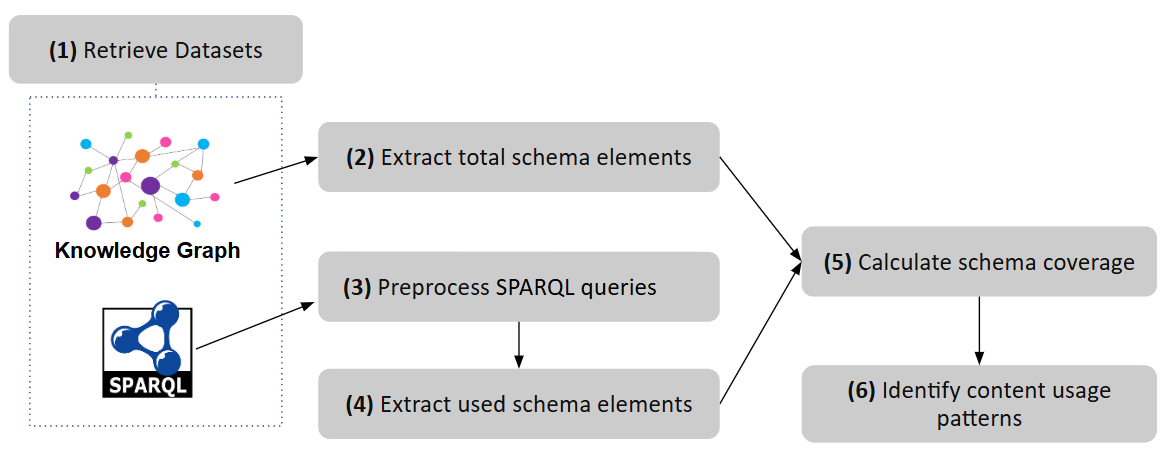
\includegraphics[width=0.8\textwidth]{image14.png} 
    \caption{Workflow of the proposed method }
    \label{fig:l1}
\end{figure}


\subsection{Datasets}

\textbf{RDF KGs.} Given that our analysis spans a period of Wikidata SPARQL query logs from 2017 to 2018, we downloaded a version of Wikidata from 2017 and 2018, as these are the closest versions available to the log period. This ensures maximum alignment of schema and query logs. We use both versions to investigate how the SPARQL schema coverage changes with the evolution of the Wikidata KG. We downloaded two versions of Wikidata from the Internet Archive\footnote{Wikidata version 2017: \url{https://archive.org/download/wikibase-wikidatawiki-20170821} and Wikidata version 2018: \url{https://archive.org/download/wikibase-wikidatawiki-20180205}}, and hosted them on Blazegraph on a local server. 

For Bio2RDF KG \cite{belleau2008bio2rdf}, the analysis covers two periods of SPARQL query logs: one beginning in 2013 and the other in 2019. However, due to the unavailability of datasets from these years, we instead use the current 2024 public endpoint\footnote{\url{https://Bio2RDF.org/sparql/}}.

\textbf{SPARQL Query Logs. }
The query logs are primarily retrieved from the Linked SPARQL Queries Dataset (LSQ) 2.0 endpoint\footnote{\url{https://lsq.data.dice-research.org/sparql}} using the query illustrated in Listing \ref{lst:SPARQL_query}. This query extracts the text and execution time of queries from 24 datasets in LSQ 2.0 \cite{stadler2024lsq}, including 23 Bio2RDF datasets and one Wikidata query dataset.
Furthermore, we downloaded Bio2RDF logs from Dumontier’s lab repository\footnote{\url{https://download.dumontierlab.com/Bio2RDF/logs/}} and Wikidata queries (all queries and organic queries for interval 1 and interval 7) from the International Center for Computational Logic\footnote{\url{https://iccl.inf.tu-dresden.de/web/Wikidata_SPARQL_Logs/en}}.

Among the many KGs available through LSQ, we selected Bio2RDF for two reasons. First, it is a domain-specific (life-sciences) KG with a compact, OWL-style schema, which contrasts sharply with the broad, general-purpose, and very large schema of Wikidata; comparing the two lets us study usage across two extremes of schema scale and design. Second, large Bio2RDF logs are available to us, including logs that retain user-agent information and therefore permit the organic/robotic split. The number of queries per dataset is substantial (ranging from $\sim$0.2 million to $\sim$81 million; full counts are reported in Tables~\ref{tab:1} and \ref{tab:2}), and we relate coverage to this sampling effort explicitly in Section~\ref{s4}.

The interval boundaries are not chosen by us; they are inherited from the upstream releases. For Wikidata, intervals~1 and~7 are the two intervals of the ICCL/Dresden release that provide the organic/robotic partition together with sufficient volume, and they bracket an approximately one-year span (2017 vs.\ 2018) that aligns with the 2017 and 2018 KG dumps we host. For Bio2RDF, the 2013 and 2019 periods correspond to the two log dumps available (LSQ and the Dumontier-lab repository, respectively). Because these periods differ in length, all frequency analyses use \emph{time-normalized} counts (Section~\ref{sec:s61}), where one month is defined as a fixed 30-day period and a log's duration in months is computed as $(\text{end date}-\text{start date})/30$ days.


\begin{center}
\begin{minipage}{0.8\textwidth}  % Adjust the width as needed
\begin{lstlisting}[label={lst:SPARQL_query},linewidth=\linewidth, caption={The templated SPARQL query against the LSQ SPARQL endpoint to retrieve SPARQL queries for selected datasets.}]
PREFIX lsqv: <http://lsq.aksw.org/vocab#>
PREFIX prov: <http://www.w3.org/ns/prov#>

SELECT DISTINCT ?text ?timeStamp

FROM <http://lsq.aksw.org/{dataset_name}>

WHERE {
    ?query  lsqv:text          ?text .
    ?query  lsqv:hasRemoteExec ?re .
    ?re     prov:atTime        ?timeStamp .
}
\end{lstlisting}
% \label{lst:SPARQL_query}
\end{minipage}
\end{center}


We implemented the method in \cite{bielefeldt2018practical, malyshev2018getting} to classify queries as organic or robotic based on the agent who executed the query. The Bio2RDF log2019 dataset includes user agent information, enabling us to generate the Bio2RDF organic and robotic log2019 subsets. The criteria used for classification are as follows:

\textbf{Organic:} If the user agent string contains indicators commonly associated with web browsers, such as "Mozilla," "Chrome," "Safari," "Firefox," "Edge," or "Opera," it was classified as organic. These are typically representative of human users.

\textbf{Robotic:} Entries whose user agent lacks browser indicators were classified as robotic. In practice these agents carry terms such as "Apache," "HttpClient," "Crawler," "sparqlwrapper," "python," or "Java," which are linked to automated scripts or bots; however, the operational rule is the complement of the organic test (any non-browser, non-empty agent), so that agents not matching a fixed keyword list are still treated as robotic rather than discarded.

\textbf{No agent:} A small number of entries carry no user-agent string and cannot be assigned to either class; they are excluded from the organic/robotic split.

\subsection{Extracting Total Schema Elements}

In this study, the \emph{schema} of a KG is the set of its distinct \emph{types} (classes) and \emph{predicates}. A \emph{schema element} is one such type or predicate. A \emph{schema (type) pattern} is a triple pattern at the schema level, $(\text{type}_1,\ \text{predicate},\ \text{type}_2)$, i.e., an edge of the schema graph connecting instances of $\text{type}_1$ to instances of $\text{type}_2$ via $\text{predicate}$. We extract these schema elements directly from the data of each KG, because neither KG ships a single authoritative schema document that matches the deployed data.

Listing~\ref{lst:l2} presents the pseudocode and queries used to extract the schema of a KG. The extraction process involves two main queries. Query~1 (line 7 in Listing~\ref{lst:l2}) retrieves all types, while Query~2 (line 13 in Listing~\ref{lst:l2}) extracts relationships between instances of different types. Using two optimized queries instead of a single complex query improved performance in large KGs, preventing timeout issues. For a few types, Query~2 still encountered timeouts due to the high number of instances and relationships; in such cases, simplified queries were used to mitigate the issue.

For Bio2RDF and Wikidata, the properties used in these queries differ. In Bio2RDF, \texttt{rdf:type} and \texttt{rdfs:subClassOf} are used, whereas Wikidata employs \texttt{wdt:P31} (\emph{instance of}) and \texttt{wdt:P279} (\emph{subclass of}) as their equivalents. Additionally, since Wikidata lacks subgraphs in its architecture, the ``Graph'' component is omitted from Query~2 when applied to Wikidata. For Bio2RDF we additionally keep only IRIs that match the Bio2RDF vocabulary template \url{http://Bio2RDF.org/DATASET_vocabulary:SCHEMA_ELEMENT} (excluding the generic \texttt{:Resource}), which yields OWL-style class and property IRIs.

\paragraph{\textbf{What counts as a ``class'' in Wikidata.}} Bio2RDF follows a classical ontology design in which classes and properties have dedicated vocabulary IRIs, so extracting them is unambiguous. Wikidata is different: properties are declared explicitly, but ``classes'' exist only informally, as ordinary items that happen to be used as the object of \texttt{wdt:P31} or \texttt{wdt:P279}. We therefore adopt a \emph{data-driven operationalization}: an item is treated as a type if it appears as the object of \texttt{wdt:P31} or \texttt{wdt:P279}. We stress that this is an operational choice, not a claim about ontological class-hood, which is genuinely contested in Wikidata \cite{brasileiro2016applying,piscopo2018who,patelschneider2024class}. Two consequences follow that we account for in the analysis and discussion (Section~\ref{s5}): (i) \texttt{wdt:P279} has subproperties, so restricting to it under-counts class-like elements; and (ii) some Wikidata domains consist almost entirely of class-like items with few or no instances, so the extracted type set is heterogeneous, mixing heavily instantiated classes with class-like individuals. We distinguish \emph{instantiated} classes (objects of \texttt{wdt:P31}, which by construction have at least one instance) from purely hierarchical items where this distinction matters, and we report a singleton-sensitivity check to bound the effect of one-off (possibly erroneous) uses.

\paragraph{\textbf{Worked example.}} Consider the two example queries from the Wikidata Query Service. The first, \texttt{SELECT ?cat WHERE \{ ?cat wdt:P31 wd:Q146 \}} (house cats), references the predicate \texttt{P31} and the type \texttt{Q146}; both are extracted as used schema elements. The second, \texttt{?horse wdt:P31/wdt:P279* wd:Q726} (horses and their subclasses), references the predicates \texttt{P31} and \texttt{P279} and the type \texttt{Q726}; these three are extracted. Note that the \texttt{wdt:P279*} closure means the query also retrieves subclasses of horse (e.g.\ \emph{racehorse}, \texttt{Q2442470}), but those subclass IRIs are \emph{not} written in the query text and are therefore not counted as explicitly referenced (we return to this distinction in Section~\ref{s3}.4 and Section~\ref{s5}).

The schema for any Bio2RDF dataset follows a specific URL template: \url{http://Bio2RDF.org/DATASET_vocabulary:SCHEMA_ELEMENT}. Therefore, any URLs retrieved from query execution that do not adhere to this template are excluded from the final schema elements set.


\begin{center}
\begin{minipage}{0.76\textwidth} % Adjust width here (e.g., 0.9 for 90% of text width)
\begin{lstlisting}[label={lst:l2},caption={Pseudocode to extract KG schema. KG schema extraction is consist of two queries, Query 1 and Query 2.}]
for graph in the KG:
        for each property in ['type_property', 'subclass_property']:
            Execute Query_1 to get subject_types
            for each subject_type and property in ['type_property', 'subclass_property']:
                execute Query_2 
                
Query_1:
SELECT DISTINCT ?subject_type
    WHERE {
        GRAPH <{graph}> {
            ?s {property} ?subject_type . } }

Query_2:
SELECT DISTINCT subject_type ?p ?object_type
WHERE {
    GRAPH <{graph}> {
        ?s {property} {subject_type} .
        ?s ?p ?o .
        ?o {property} ?object_type .  }} 
                    
\end{lstlisting}
\end{minipage}
\end{center}

\subsection{Preprocessing SPARQL Queries}

We extract unique SPARQL queries and store them along with their respective execution counts. Two queries are considered identical when their text is identical after collapsing runs of whitespace (spaces, tabs, and newlines) to a single space and trimming leading/trailing whitespace; we do not otherwise reformat the queries at this stage. We count over \emph{unique} queries because our questions concern the \emph{diversity} of schema elements that users and tools query, and deduplication prevents a small number of very high-frequency automated queries from dominating the distribution. We note that repetition is itself a meaningful signal of demand; deduplication is a deliberate choice to measure intent diversity rather than execution volume, and a complementary volume-weighted analysis is a natural extension. Before parsing, we preprocess the queries to ensure proper syntax and facilitate accurate parsing. First, we incorporate essential RDF syntax prefixes (such as \texttt{rdf}, \texttt{rdfs}, and \texttt{owl}) since some queries lack explicit prefix declarations. While Virtuoso pre-registers these prefixes—allowing users to omit them—our parser, 'sparqljs'\footnote{https://www.npmjs.com/package/sparqljs}, does not support this feature. Therefore, we add the necessary prefixes to all queries to ensure proper parsing.

Next, we normalize the queries for parsing. Crucially, this normalization is performed \emph{before} deduplication, so that queries differing only in incidental HTTP artifacts collapse to a single unique query. Specifically, we (i) fully percent-decode the query text (not only \texttt{\%3A}); (ii) remove the trailing chain of HTTP query-string parameters that the log capture appended to the SPARQL text (queries were submitted as \texttt{GET /sparql?query=<SPARQL>\&format=...\&timeout=...\&callback=...}); we strip a terminal run of \texttt{\&key=value} segments, anchored to the end of the string so that IRIs containing \texttt{\&} mid-query are not affected; and (iii) collapse runs of whitespace. We do \emph{not} rewrite the empty/relative IRI \texttt{<>}: doing so (e.g., to a variable) would change query semantics, so instead relative IRIs are resolved by supplying the parser a base IRI, as the Virtuoso endpoint itself does. Failing to strip the appended parameters causes many syntactically valid queries to be rejected; the dominant leaked parameter was \texttt{\&callback} (from JSONP/visualization clients), which earlier processing overlooked.
% fix instances of missing spaces (e.g., replacing \texttt{GROUP BY ?rOFFSET 0} with \texttt{GROUP BY ?r OFFSET 0}),



After preprocessing, we parse the queries using the 'sparqljs', a SPARQL 1.1 parser implemented in JavaScript to eliminate queries that are not syntactically valid and get the parse tree of the queries for content extraction. A parse tree represents the syntactic structure of a query, breaking it down into its components, such as subjects, predicates, and objects.  We standardize variable names, as demonstrated in Figure \ref{fig:l2}. Three equivalent queries that differ only in their variable names e.g., ?drug, ?compound, and ?s1, are standardized to ?var1. We distinguish variables from actual entities by substituting variable names with placeholders like 'varX'. The same preprocessing and variable standardization are applied identically to both the Bio2RDF and Wikidata logs. The output of this preprocessing is unique, normalized, valid queries.

\begin{figure}
    \centering
    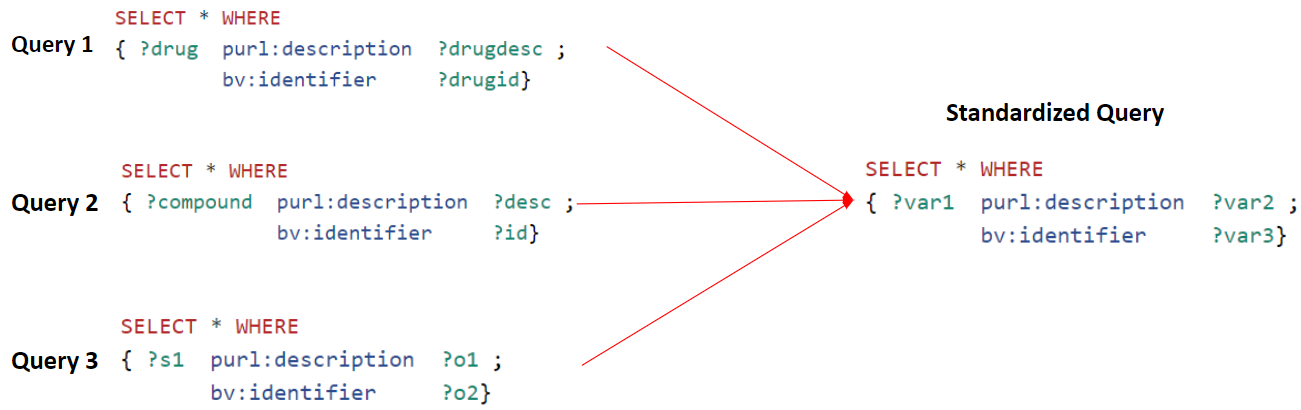
\includegraphics[width=0.8\textwidth]{image17.png} 
    \caption{Variable standardization. ?drug, ?compound, and ?s1, are standardized to ?var1.}
    \label{fig:l2}
\end{figure}
\subsection{Extracting Used Schema Elements }\label{sec:used}
We write a Python script to extract ``used schema elements'' from the parse trees of the queries. We first identify the subject, predicate, and object IRIs within each query's parse tree. Then, we determine the intersection of these IRIs with the total schema elements that were retrieved earlier.

\paragraph{\textbf{What we mean by ``used''.}} Throughout, a schema element is counted as \emph{used} if it is \emph{explicitly referenced}, i.e., its IRI is written in the query text. We deliberately adopt this explicit-reference notion rather than a closure- or answer-based one. As illustrated by the horse example in Section~\ref{s3}.2, a query containing \texttt{wdt:P31/wdt:P279* wd:Q726} explicitly references only \texttt{P31}, \texttt{P279}, and \texttt{Q726}; the subclasses of horse that the property path traverses at evaluation time (e.g.\ \emph{racehorse}) contribute to the \emph{answers} but are not named in the query, and a similar effect arises with property hierarchies. Explicit reference is the appropriate notion for this paper's motivations: documentation, schema and interface design, autocomplete, and deprecation decisions all act on the elements that users and tools actually \emph{write}, not on the transitive closure a query happens to traverse. We quantified how often the two notions could diverge by measuring property-path usage (the \texttt{*}/\texttt{+} operators that trigger transitive traversal): property paths appear in only about 1\% of valid Bio2RDF organic queries (98 of 8,140), but in 21.1\% of Wikidata organic queries in 2017 (18,705 of 88,491) and 13.7\% in 2018 (25,351 of 185,443). The explicit-reference and closure-based notions therefore coincide for nearly all Bio2RDF queries, whereas for Wikidata a non-trivial fraction of queries use paths whose traversed subclasses/subproperties a closure-based notion would additionally credit. A complementary closure-based notion of ``effective usage'', which would attribute usage to every subclass and subproperty that contributes answers, is a substantial separate study that we identify as future work (Section~\ref{s5}); the figures above bound how much it could change the Wikidata results.

\subsection{Calculating Schema Coverage}
Equation \ref{eq:1} was used to calculate the SPARQL Schema Coverage (SC). This metric quantifies the proportion of the KG schema that is used by user queries. SC is the ratio of Used Schema Elements (USE) to Total Schema Elements (TSE) in the KG, multiplied by 100 to express the result as a percentage. The TSE represents the count of all distinct types and predicates in the KG, while the USE denotes the count of those classes and predicates found in user SPARQL query logs. We obtained the values for USE and TSE from the results of the previously described steps. Coverage is always reported against a \emph{clearly delimited reference set}: the numerator and denominator are derived from the same set of subgraphs (Section~\ref{s4}.1), and we report types and predicates separately (Table~\ref{tab:4}) rather than only their sum. Because the type sets of Bio2RDF and Wikidata are constructed differently (OWL-style vocabulary IRIs vs.\ the data-driven \texttt{wdt:P31}/\texttt{wdt:P279} operationalization of Section~\ref{s3}.2) and differ in scale by roughly two orders of magnitude, coverage percentages are meaningful \emph{within} a KG (across query types and time) but should not be read as a direct cross-KG comparison.
\begin{equation}
SC (\%) = \left( \frac{USE}{TSE} \right) \times 100
\label{eq:1}
\end{equation}

\subsection{Identifying Content Usage Patterns}\label{sec:s6}
Up to this point, we have introduced a method for calculating SPARQL schema coverage, which measures the proportion of schema elements in a KG that are queried. However, this metric alone does not reveal how frequently individual schema elements are used or whether their usage is consistent over time. Step six involves analyzing the frequency distribution of the schema elements, identifying frequently used elements, and detecting commonalities in robotic and organic logs, or across different time periods. Additionally, we apply statistical tests, including the Wilcoxon signed-rank test and Spearman's rank correlation coefficient, to assess the consistency and changes in the frequency and ranking of schema element usage over time. The following sections provide a detailed explanation of these methods, with the findings presented in the Results section.

\subsubsection{Frequency Distribution of Schema Elements}\label{sec:s61}
To analyze and compare the frequency distributions of schema elements across multiple datasets, we normalize the usage count of each element to account for varying time intervals. We calculate the monthly frequency of each element by dividing its total count by the log collection period expressed in months (Equation \ref{eq:2}). Here one month is a fixed 30-day period, so the normalized count has units of \emph{uses per 30-day month} (it is not dimensionless). To reduce skewness and enhance interpretability, we apply a logarithmic transformation ($\log_{10}$) to these normalized counts. Finally, we visualize the normalized frequency distribution of schema elements across different datasets to facilitate comparison.

\begin{equation}
\text{Normalized count} = \frac{\text{Total count}}{\text{log collection period}}
\label{eq:2}
\end{equation}

Before comparing the two intervals statistically, we must decide whether a parametric (normality-assuming) test is appropriate. The Shapiro--Wilk test (Equation~\ref{eq:shapiro}) assesses whether a sample plausibly comes from a normal distribution; we use it purely as a precondition check. We apply it to the per-element \emph{change} in normalized usage frequency between the two intervals (defined below). We emphasize that normality here is a property of these numeric differences (real numbers, naturally ordered), not of any ordering over the schema elements themselves.

\begin{equation}
SW = \frac{\left( \sum_{i=1}^n a_i x_i \right)^2}{\sum_{i=1}^n (x_i - \bar{x})^2}
\label{eq:shapiro}
\end{equation}

where the \( x_i \) are the ordered sample values, \( \bar{x} \) is the sample mean, and the \( a_i \) are the Shapiro--Wilk coefficients, i.e., tabulated constants derived from the expected values and covariances of the order statistics of a standard-normal sample of size \( n \). In our case each \( x_i \) is, for one schema element common to both intervals, the change in its normalized monthly usage frequency from the first interval to the second (interval-2 value minus interval-1 value).


The test returned $p \approx 0$ for both the Wikidata and Bio2RDF interval pairs, so the per-element changes are not normally distributed. We therefore use the non-parametric Wilcoxon signed-rank test (Equation~\ref{eq:wilcoxon}), which compares the same schema element measured in two intervals (a paired design) without assuming normality, to test whether usage frequencies shifted significantly between the two intervals.

\begin{equation}
W = \sum_{i=1}^n \text{sign}(d_i) R_i
\label{eq:wilcoxon}
\end{equation}

where \(d_i\) is the difference between the usage frequency of schema elements (in two intervals), \( \text{sign}(d_i) \) is the sign of \(d_i\), and \(R_i\) is the rank of the absolute differences.


\paragraph{\textbf{Changes in Used Schema Element Ranking.}}
The Wilcoxon test addresses changes in usage \emph{magnitude}; we separately ask whether the relative \emph{popularity ranking} of schema elements is stable over time. We rank elements by their normalized usage frequency within each interval (rank 1 = most frequently used) and compute Spearman's rank correlation coefficient (\( \rho \)) (Equation~\ref{eq:4}) between the two rankings. Spearman's \( \rho \) is the Pearson correlation of the ranks; it summarizes in a single number in \([-1,1]\) whether elements that were popular in one interval remained popular in the other, and it is distribution-free, which suits our non-normal data. Here \( d_i \) is the difference between the ranks of schema element \( i \) in the two intervals, and \( n \) is the number of common schema elements \cite{spearman1961proof}. We use Spearman's \( \rho \) as a compact measure of temporal \emph{stability}, complementing the Wilcoxon test.
\begin{equation}
\rho = 1 - \frac{6 \sum d_i^2}{n(n^2 - 1)}
\label{eq:4}
\end{equation}

% To measure the proportion of schema element pairs that maintain their relative rank ordering between the two intervals, we calculate the concordance index (equation~\ref{eq:5}), where concordant pairs are defined as a pair of schema elements \( (i, j) \) that their relative ranks are the same in both intervals.

% \begin{equation}
%     \text{C-index} = \frac{\text{Number of concordant pairs}}{\text{Total number of pairs}}
%     \label{eq:5}
% \end{equation}


\subsubsection{Frequent Schema Elements} \label{sec:s62}
We analyze the most frequently queried schema types from robotic and organic logs of Wikidata and Bio2RDF to identify common elements that persist across different time intervals and log types. This focus on the most frequent elements is similar in spirit to the predicate-frequency analysis of Bonifati et al.\ \cite{bonifati2019navigating}, to which we add the temporal and organic/robotic dimensions. While our ranking analysis of all schema elements reveals broad usage dynamics and temporal shifts, we're particularly interested in determining whether a subset of frequently accessed elements remains consistently popular over time, indicating their significance as "core" elements of the KG. The presence of a stable core across the datasets would suggest that these elements are central to the KG’s utility, regardless of the query time or type. This frequent-element analysis is computed over schema \emph{types} (classes); predicates, whose frequency distribution is dominated by a few generic relations, are analyzed separately. To investigate the stable core, we first examine the top 10 schema types in each dataset, as they represent the most frequently queried components, as well as the top 50 types. The top 50 threshold strikes a balance by providing a more comprehensive view of usage patterns compared to the top 10 while still avoiding the inclusion of many low-frequency types. For example, in Wikidata 2017, the frequency for types ranked 51 to 3560 ranges from 149 to 1, whereas the top 50 types have frequencies between 6,962 and 150. To analyze schema usage patterns, we visualize frequently queried schema elements and identify common elements across datasets, log types, and time intervals. This approach aims to determine whether there is a set of core schema elements that drives query activity in these KGs.


\paragraph{\textbf{Pairwise Schema Type Usage of Bio2RDF.}}
Bio2RDF consists of 26 interconnected subgraphs, each representing a distinct dataset with its own vocabulary. These subgraphs are linked through various predicates. For example, the \url{ctd_vocabulary:Gene-Disease-Association} type from the "ctd" subgraph and the \url{ncbigene_vocabulary:Resource} from the "ncbigene" subgraph are linked by the predicate \url{ctd_vocabulary:gene}, establishing a relationship between the two elements. A typical triple pattern representing the connection between two distinct subgraphs is: \sloppy \texttt{?schema\_Type\_from\_first\_subgraph ?predicate ?schema\_Type\_from\_second\_subgraph}. This relationship is referred to as a "pairwise schema type pattern."

Bio2RDF’s subgraph organization enables an analysis of how frequently queries capture relationships between schema types from different subgraphs. However, since Wikidata does not have an explicit subgraph structure, this type of analysis is not applicable to its dataset. To investigate this type of usage, we conduct an experiment comparing Bio2RDF query logs from 2013 and 2019 to determine how often datasets (or subgraphs) were integrated in queries to retrieve more complex information. The approach consists of two main steps:

\textbf{Identifying total pairwise schema type patterns.} We extract all possible pairwise schema type patterns from the Bio2RDF schema, covering 17 subgraphs in log\_2013 and 26 subgraphs in log\_2019.


\textbf{Identifying pairwise schema type pattern occurrences in logs.} We analyze the triple patterns within queries to identify occurrences of these pairwise schema type patterns. For each dataset, we construct a matrix where both rows and columns represent schema type subgraphs. Each cell in the matrix corresponds to a specific pair of subgraphs, and its value indicates the frequency of the pattern in the queries.
By conducting this analysis, we aim to discover how often queries integrate information across Bio2RDF subgraphs and how this usage has evolved over time.

\section{Results}\label{s4}
In this section, we describe the results of the various steps in the method, including the retrieval of datasets, the pre-processing of SPARQL queries, the extraction of all schema elements, the extraction of the schema elements used, the calculation of the SPARQL schema coverage, and the analysis of usage patterns.

\subsection{Dataset Retrieval }
Table \ref{tab:1} provides an overview of the datasets retrieved for analysis, including the logs from Bio2RDF and Wikidata KGs for multiple periods and query types. We use a single naming convention of the form \emph{KG-agenttype-period[-interval] (KG version)}; for example, \emph{Bio2RDF-all-2013} is the full 2013 Bio2RDF log and \emph{Wikidata-organic-2017-int1} is interval~1 of the 2017 Wikidata organic log. The \emph{Bio2RDF-all-2013} log originates from LSQ and spans 16.79 months, from May 2013 to September 2014, containing 31,950,877 queries. This dataset lacks user-agent information and only includes the \texttt{lsqv:hostHash} property, an anonymized hash of the host or IP address issuing each query; consequently it cannot be split into organic and robotic. The second dataset, \emph{Bio2RDF-all-2019}, covers a longer period of 29.93 months, from January 2019 to July 2021. It comprises 3,880,960 log entries. Of these, 3,212 are server-side log lines that contain no SPARQL query, leaving 3,877,748 SPARQL queries. This dataset retains user-agent information, allowing us to separate robotic (3,816,776) and organic (56,736) queries; a further 7,427 queries lack user-agent information and are excluded from the split.

Wikidata logs contain both organic and robotic queries. The \emph{Wikidata-organic-2017-full} log spans 9.43 months, from June 2017 to March 2018, and consists of 3,298,254 organic queries. The shorter, interval-based slices used for the temporal comparison were collected over only 0.88 months each: \emph{Wikidata-organic-2017-int1} and \emph{Wikidata-organic-2018-int7} comprise 192,331 and 872,556 organic queries, respectively, while \emph{Wikidata-robotic-2017-int1} and \emph{Wikidata-robotic-2018-int7} contain 59,355,579 and 81,339,186 robotic queries, respectively.

\begin{table}[h!]
\centering
\caption{Results of the data retrieval step. Datasets follow the naming convention \emph{KG-agenttype-period[-interval]}; ``All'' denotes the union of organic and robotic queries (not a superset of any single row).}
\label{tab:1}
\begin{tabular}{l|r|l|r} 
\hline
\textbf{Dataset} & \#\textbf{Queries} & \textbf{log collection period} & \textbf{Duration (months)} \\ \hline
Bio2RDF All log2013 & 31,950,877 & 2013-05-05 to 2014-09-28 & 16.79 \\ 
Bio2RDF All log2019 & 3,880,960  & 2019-01-07 to 2021-07-06 & 29.93 \\ 
Bio2RDF robotic log2019 & 3,816,776  & 2019-01-07 to 2021-07-06 & 29.93 \\ 
Bio2RDF organic log2019 & 56,736 & 2019-01-07 to 2021-07-06 & 29.93 \\ 
Wikidata All organic log2017 & 3,298,254 & 2017-06-11 to 2018-03-25 & 9.43 \\ 
Wikidata robotic log2017 & 59,355,579 & 2017-06-12 to 2017-07-09 & 0.88 \\ 
Wikidata robotic log2018 & 81,339,186 & 2018-02-26 to 2018-03-25 & 0.88 \\ 
 Wikidata organic log2017&
192,331&
2017-06-12 to 2017-07-09&
0.88\\
Wikidata organic log2018&
872,556&
 2018-02-26 to 2018-03-25&
0.88\\
\hline
\end{tabular}
\end{table}

During our analysis in 2024, the Bio2RDF SPARQL endpoint contained 26 subgraphs/datasets. However, the Bio2RDF log2013 and Bio2RDF log2019 datasets do not contain query logs corresponding to all 26 subgraphs. Figures \ref{fig:l3} and \ref{fig:l4} provide details through Venn diagrams: Figure \ref{fig:l3} illustrates the overlap between the Bio2RDF log2013 datasets and the KG subgraphs, while Figure \ref{fig:l4} represents the Bio2RDF log2019 datasets compared to the KG subgraphs in the 2024 endpoint. This comparison highlights the importance of using a consistent reference set when calculating schema coverage (Equation \ref{eq:1}). That is, the numerator and denominator (i.e., used and total schema elements) should be derived from the same set of datasets, ensuring alignment between KG subgraphs and log datasets.

The Venn diagram in Figure \ref{fig:l3} compares the datasets included in Bio2RDF log2013 with the subgraphs in Bio2RDF KG2024. The left oval represents datasets unique to Bio2RDF log2013. The overlapping section in the center lists 17 datasets common to both Bio2RDF log2013 and Bio2RDF KG2024. The right oval represents datasets unique to Bio2RDF KG2024.


The Venn diagram in Figure \ref{fig:l4} compares the datasets included in Bio2RDF log2019 with the subgraphs in Bio2RDF KG2024. The left oval represents datasets unique to Bio2RDF log2019. The overlapping section in the center lists 22 datasets common to both Bio2RDF log2019 and Bio2RDF KG2024. The right oval represents datasets unique to Bio2RDF KG2024. 

The  dataset "Bio2RDF" in log2019 refers to the logs of a general endpoint for all subgraphs and may include queries to the HP, ECO, APO, and GO subgraphs. This is because, historically, Bio2RDF maintained a distinct SPARQL endpoint for each subgraph. Later, a single general endpoint was introduced to host all subgraphs for querying.
 

\begin{figure}
    \centering
    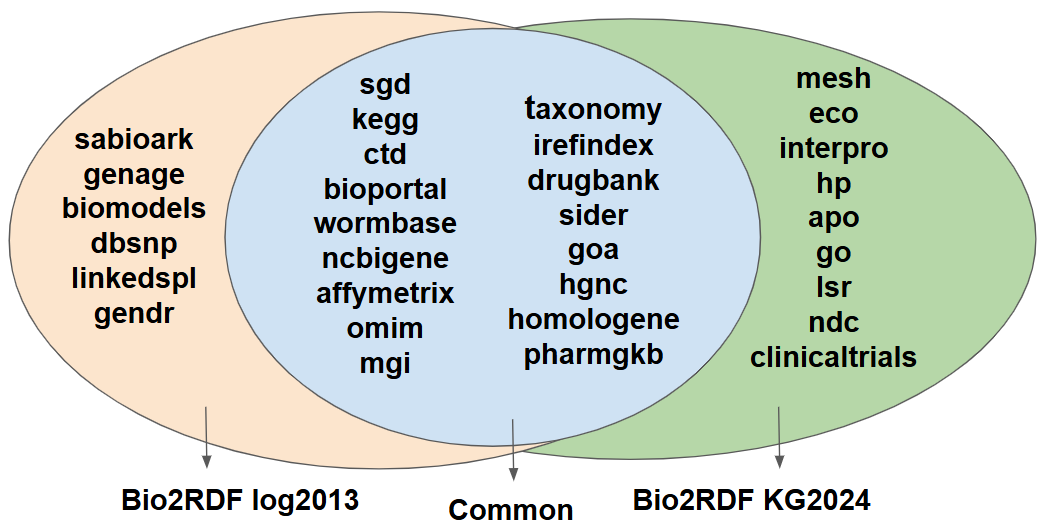
\includegraphics[width=0.53\textwidth]{image9.png} 
    \caption{Venn diagram illustrating the overlap  between the Bio2RDF log2013 datasets and the Bio2RDF KG 2024
}
    \label{fig:l3}
\end{figure}

\begin{figure}[htbp]
    \centering
    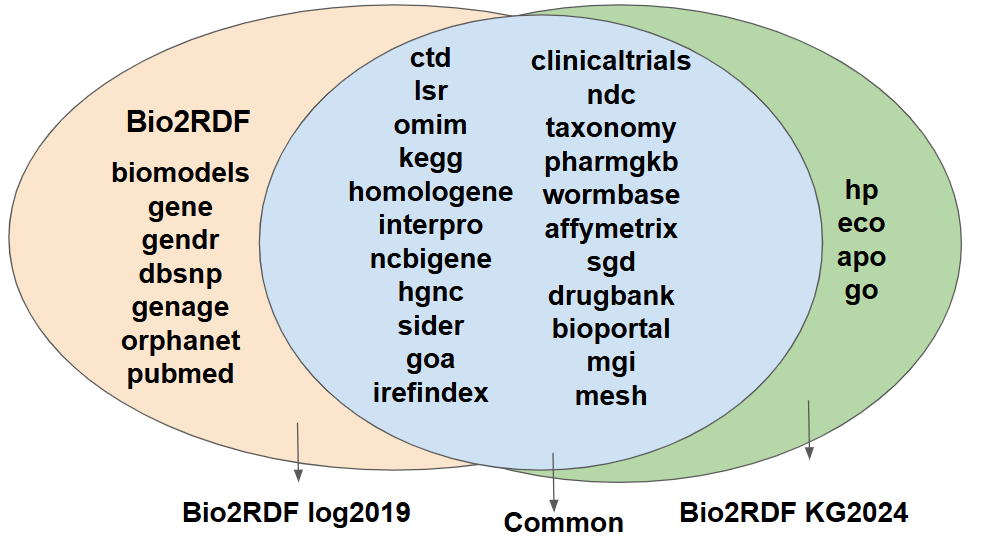
\includegraphics[width=0.55\textwidth]{image8.png} 
    \caption{ Venn diagram illustrating the overlap between the Bio2RDF log2019 datasets and the Bio2RDF KG 2024
}
     \label{fig:l4}
\end{figure}


\subsection{Extracting Total Schema Elements}
Table \ref{tab:3} presents the statistics of total schema elements across different KG versions. Initially, the Bio2RDF schema comprised 166,444 unique types. After excluding types that do not adhere to the template \url{http://Bio2RDF.org/DATASET_vocabulary:SCHEMA_ELEMENT}',' 545 types remain. A further refinement, by excluding elements with the template \url{'http://Bio2RDF.org/DATASET_vocabulary:Resource,'} reduces the count to 350 types and 195 predicates, distributed across 26 subgraphs within the Bio2RDF KG on the current endpoint (2024). Out of these 26 subgraphs, only 17 have corresponding query logs available in the Bio2RDF log2013 dataset, as depicted in Figure \ref{fig:l3}. These 17 subgraphs contain 270 types and 129 predicates, in total 399 schema elements.

As represented in Table \ref{tab:3}, the Wikidata KG version 2017 contains 103,380 types, whereas the Wikidata KG version 2018 contains 97,470 types, reflecting a reduction in the number of schema types. These results illustrate the variability in schema complexity with Wikidata exhibiting a larger and more diverse set of schema elements compared to Bio2RDF.
\begin{table}[ht]
\centering
\caption{Total schema elements Statistics per KG version}
\label{tab:3}
\resizebox{\textwidth}{!}{
\begin{tabular}{l|r|r|r|r}
\hline
Source & Bio2RDF KG2024 (17 subgraphs) & Bio2RDF KG2024 (26 subgraphs) & Wikidata KG2017 & Wikidata KG2018 \\
\hline
Total number of distinct Elements & 399 & 545 & 104,314 & 98,462 \\
Number of distinct Types & 270 & 350 & 103,380 & 97,470 \\
Number of distinct Predicates & 129 & 195 & 934 & 992 \\
\hline
\end{tabular}
}
\end{table}


\subsection{Preprocessing SPARQL Queries}
Table \ref{tab:2} summarizes the number of queries (\#Queries), unique queries (\#Unique), queries with incorrect syntax (\#Failed to parse), and unique syntactically valid queries (\#Valid) across all datasets. We emphasize the Bio2RDF~2019 rows: with the corrected preprocessing, the number of valid queries is far higher than under the earlier pipeline (e.g., for robotic~2019, 1{,}034{,}831 vs.\ 627{,}314), because previously the appended HTTP parameters had caused a large share of well-formed queries to be discarded. The LSQ-sourced Bio2RDF~2013 and the Dresden-sourced Wikidata logs were cleanly extracted and reproduce closely (validity rates of 99.8\% and $>$99.9\% respectively), confirming that the parsing defect was specific to the raw Bio2RDF~2019 server logs and does not affect the schema-coverage results, which are computed over the same valid queries.

% We reviewed the 416,896 queries in the Bio2RDF log 2019 that failed to parse. Approximately 300,000 of the 416,896 failures were simple templates with varying LIMIT and OFFSET values, as shown in Listing \ref{lst:third_list} 6 with a syntactic error. More than 1,819 of these queries were not SPARQL queries at all; rather, they were plain text, mostly in English. For example, one such message reads: "I love your blog... very nice colors \& theme. Did you make ...". Interestingly, the execution agent for these queries is Mozilla, rather than Java, Python, or any web crawler. Nine queries contained only the string "/sparql." 
% \begin{center}
% \begin{minipage}{0.76\textwidth} % Adjust width here (e.g., 0.9 for 90% of text width)
% \begin{lstlisting}[caption={The templated SPARQL query against the LSQ SPARQL endpoint to retrieve SPARQL queries for selected datasets.}]
% -- Query 1

%     SELECT ?r (COUNT(*) AS ?count) WHERE { ?r ?s ?o } 
%     OFFSET 177863205 LIMIT 1000 
%     GROUP BY ?rOFFSET 0 LIMIT 10000
    
%  -- Query 2
 
%     SELECT ?r (COUNT(*) AS ?count) WHERE { ?r ?s ?o } 
%     OFFSET 62950773 LIMIT 1000 
%     GROUP BY ?rOFFSET 0 LIMIT 10000
    
% -- Query 3

%     SELECT ?r (COUNT(*) AS ?count) WHERE { ?r ?s ?o } 
%     OFFSET 85005378 LIMIT 1000 
%     GROUP BY ?rOFFSET 0 LIMIT 10000

% \end{lstlisting}
% \label{lst:third_list}
% \end{minipage}
% \end{center}

\begin{table}[ht]
\centering
\caption{Results of parsing and validating the query logs, regenerated with the
corrected preprocessing (full HTTP query-string parameter stripping applied before
deduplication, base-IRI resolution of relative IRIs). \#Failed-to-parse $=$ \#Unique
$-$ \#Valid. \#Valid is computed with a SPARQL~1.1 parser (sparqljs). The Bio2RDF~2019
rows change substantially relative to earlier processing because appended HTTP
parameters (notably \texttt{\&callback}) had previously caused many valid queries to be
rejected; the LSQ-sourced (Bio2RDF~2013) and Dresden-sourced (Wikidata) logs were
already cleanly extracted and reproduce. The Bio2RDF~2013 figures use the executed-query
set (queries with a recorded remote execution).}
\label{tab:2}
\begin{tabular}{l|r|r|r|r}
\hline
Dataset & \#SPARQL Queries & \#Unique & \#Failed to parse & \#Valid \\
\hline
Bio2RDF All log2013 & 31,950,877 & 1,519,681 & 2,521 & 1,517,160 \\
Bio2RDF All log2019 & 3,880,939 & 1,050,616 & 9,950 & 1,040,666 \\
Bio2RDF robotic log2019 & 3,824,203 & 1,040,356 & 5,525 & 1,034,831 \\
Bio2RDF organic log2019 & 56,736 & 12,579 & 4,439 & 8,140 \\
Wikidata All organic log2017 & 3,530,948 & 859,290 & 321 & 858,969 \\
Wikidata robotic log2017 & 59,355,579 & 8,234,089 & 20 & 8,234,069 \\
Wikidata robotic log2018 & 81,339,186 & 18,939,743 & 86 & 18,939,657 \\
Wikidata organic log2017 & 192,330 & 88,514 & 23 & 88,491 \\
Wikidata organic log2018 & 872,555 & 185,478 & 35 & 185,443 \\
\hline
\end{tabular}
\end{table}


\subsection{Extracting Used Schema Elements} 
Table \ref{tab:4} presents the statistics of used schema elements in various datasets, detailing the total number of distinct elements, types, and predicates identified in the queries. From Bio2RDF log2019\_kg2024, 529 distinct elements were extracted, comprising 334 distinct types and 195 distinct predicates. In comparison, Bio2RDF log2013\_kg2024 contains 317 distinct elements, with 227 distinct types and 90 predicates. The robotic queries for Bio2RDF log2019 match the overall log2019\_kg2024 dataset, both reporting 529 distinct elements, 334 classes, and 195 predicates, while the organic queries yield a much smaller subset of 116 elements, 58 types, and 58 predicates.

For Wikidata, log2017\_kg2017 includes 13,394 distinct elements, 12,590 classes and 804 predicates, while log2017\_kg2018 has 13,900 distinct elements, consisting of 13,054 types and 846 predicates. The robotic queries for Wikidata scale significantly larger, with robotic log2017\_kg2017 containing 59,603 elements, 58,680 types, and 923 predicates, and robotic log2018\_kg2018 reporting 59,582 elements, 58,648 types, and 934 predicates. These results illustrate significant variability in schema usage between robotic and organic logs.
\begin{table}[ht]
\centering
\caption{Used schema-element statistics. Each row is based on a \emph{pair} of datasets: a query log and the KG version it is evaluated against, written \emph{log}\_\emph{kg} (e.g.\ \emph{Bio2RDF-all-log2013\_kg2024} = the 2013 log matched against the 2024 KG). Counts are over unique normalized queries.}
\label{tab:4}
\begin{tabular}{l|r|r|r}
\hline
Dataset & Total number of distinct Elements & Number of distinct Types & Number of distinct Predicates \\
\hline
Bio2RDF All log2013\_kg2024 & 317 & 227 & 90 \\
Bio2RDF All log2019\_kg2024 & 529 & 334 & 195 \\
Bio2RDF robotic log2019\_kg2024 &  529 & 334 & 195 \\
Bio2RDF organic log2019\_kg2024 &  116 & 58 & 58 \\
Wikidata All organic log2017\_kg2017 & 13,394 & 12,590 & 804 \\
Wikidata All organic log2017\_kg2018 & 13,900 & 13,054 & 846 \\
Wikidata robotic log2017\_kg2017 & 59,603 & 58,680 & 923 \\
Wikidata robotic log2018\_kg2018 & 59,582 & 58,648 & 934 \\
Wikidata organic log2017\_kg2017 & 4,041 & 3,559 & 482 \\
Wikidata organic log2018\_kg2018 & 4,859 & 4,310 & 549 \\
\hline
\end{tabular}
\end{table}

\subsection{Calculating SPARQL Schema Coverage}
Table \ref{tab:5} presents the SPARQL schema coverage of datasets and provides insight into the extent to which schema elements of different KGs are used in SPARQL queries. Bio2RDF All log2019\_kg2024 and Bio2RDF robotic log2019\_kg2024 achieved the highest schema coverage at 97.06\%, indicating that nearly all schema elements were queried at least once. This is followed by Bio2RDF All log2013\_kg2024, which achieved a schema coverage of 79.44\%.  

In contrast, the Bio2RDF Organic log2019\_kg2024 exhibited a much lower schema coverage of 21.28\%. Similarly, the schema coverage for Wikidata robotic queries in log2017\_kg2017 and log2018\_kg2018 was moderate, at 57.13\% and 60.51\%, respectively. However, the schema coverage for Wikidata organic queries in log2017\_kg2017 and log2018\_kg2018 was significantly lower, at 12.84\% and 14.11\%, respectively.

\begin{table}[ht]
\centering
\caption{SPARQL schema coverage. Each row pairs a query log with a KG version (\emph{log}\_\emph{kg}); coverage is $\mathrm{USE}/\mathrm{TSE}\times100$ over the same reference set of subgraphs. As discussed in Sections~\ref{s3}.5 and \ref{sec:rarefaction}, these percentages are comparable within a KG but not directly across the two KGs.}
\label{tab:5}
\begin{tabular}{l|r}
\hline
Dataset & SC \\
\hline
Bio2RDF All log2013\_kg2024 & 79.44\% \\
Bio2RDF All log2019\_kg2024 & 97.06\% \\
\textbf{Bio2RDF robotic }log2019\_kg2024 & \textbf{97.06}\%\\
Bio2RDF organic log2019\_kg2024 & 21.28\% \\
Wikidata All organic log2017\_kg2017 & 12.84\% \\
Wikidata All organic log2017\_kg2018 & 14.11\% \\
Wikidata robotic log2017\_kg2017 & 57.13\% \\
\textbf{Wikidata robotic} log2018\_kg2018 & \textbf{60.51}\% \\
Wikidata organic log2017\_kg2017 & 3.87\%  \\
Wikidata organic log2018\_kg2018 & 4.93\%  \\
\hline
\end{tabular}
\end{table}



These results highlight a notable difference in schema coverage between robotic and organic queries across Bio2RDF and Wikidata datasets.
\begin{figure}
    \centering
    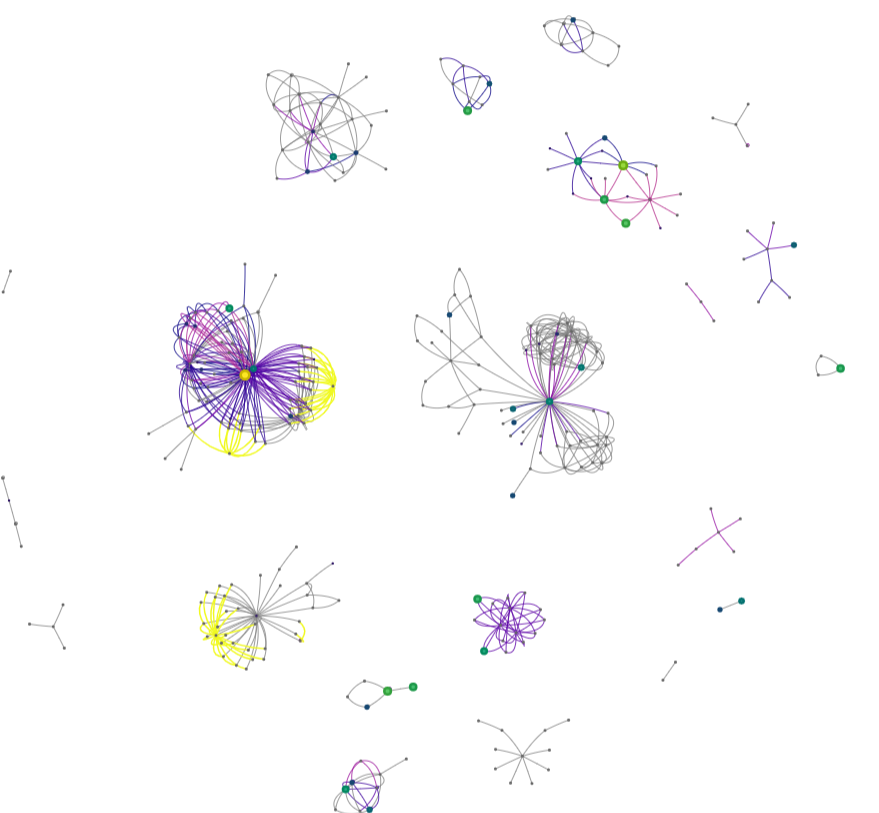
\includegraphics[width=0.6\textwidth]{image21.png} 
    \caption{Visualization of schema-element usage in \emph{Bio2RDF-organic-2019} (KG2024). Node size and color both increase with usage frequency (small/dark = rarely used, large/bright = heavily used); edge width increases with predicate usage; schema elements not used in any query are gray. The few large, bright hubs concentrate most of the usage.}
    \label{fig:l5}
\end{figure}

Figure \ref{fig:l5} illustrates the extent to which schema elements of the Bio2RDF KG are used in the organic queries of 2019. Nodes represent schema types and edges represent predicates linking instances of those types. Both the size and the color of a node encode the same quantity, its usage frequency: nodes grow larger and brighter as they are queried more often, while rarely used nodes are small and dark. Edge width likewise grows with predicate usage, and schema elements that appear in no query are shown in gray. The visualization makes the long tail visible directly: a handful of large, bright hubs (drug, gene, and disease types) concentrate the bulk of organic usage, while most of the schema remains gray and unqueried. The interactive version, with exact per-element values, is available online\footnote{\url{https://marmhm.github.io/Schema-usage-graph/}}.

\subsection{Size-Controlled Coverage: Is the Organic/Robotic Gap a Sampling Artifact?}\label{sec:rarefaction}
The coverage values in Table~\ref{tab:5} could be misleading, because organic and robotic logs differ enormously in size (Table~\ref{tab:2}), and larger samples mechanically touch more vocabulary. To separate a genuine behavioral difference from this sampling effect, we treat each occurrence of a schema element in a log as an ``individual'' and apply \emph{individual-based rarefaction} \cite{hurlbert1971nonconcept}: for the larger (robotic) log we compute the \emph{expected} number of distinct schema elements that would be recovered from a random sub-sample of the \emph{same} size as the organic log. As a complementary, sampling-size-independent check we also computed the Chao1 richness estimator \cite{chao1984nonparametric}; it points the same way (for Bio2RDF the organic estimate, $\approx$144, sits only modestly above the 116 observed, indicating little hidden richness, whereas the robotic estimate equals its observed 529). Figure~\ref{fig:rarefaction} shows the resulting rarefaction curves and Table~\ref{tab:rarefaction} the equal-effort comparison.

\begin{figure}
    \centering
    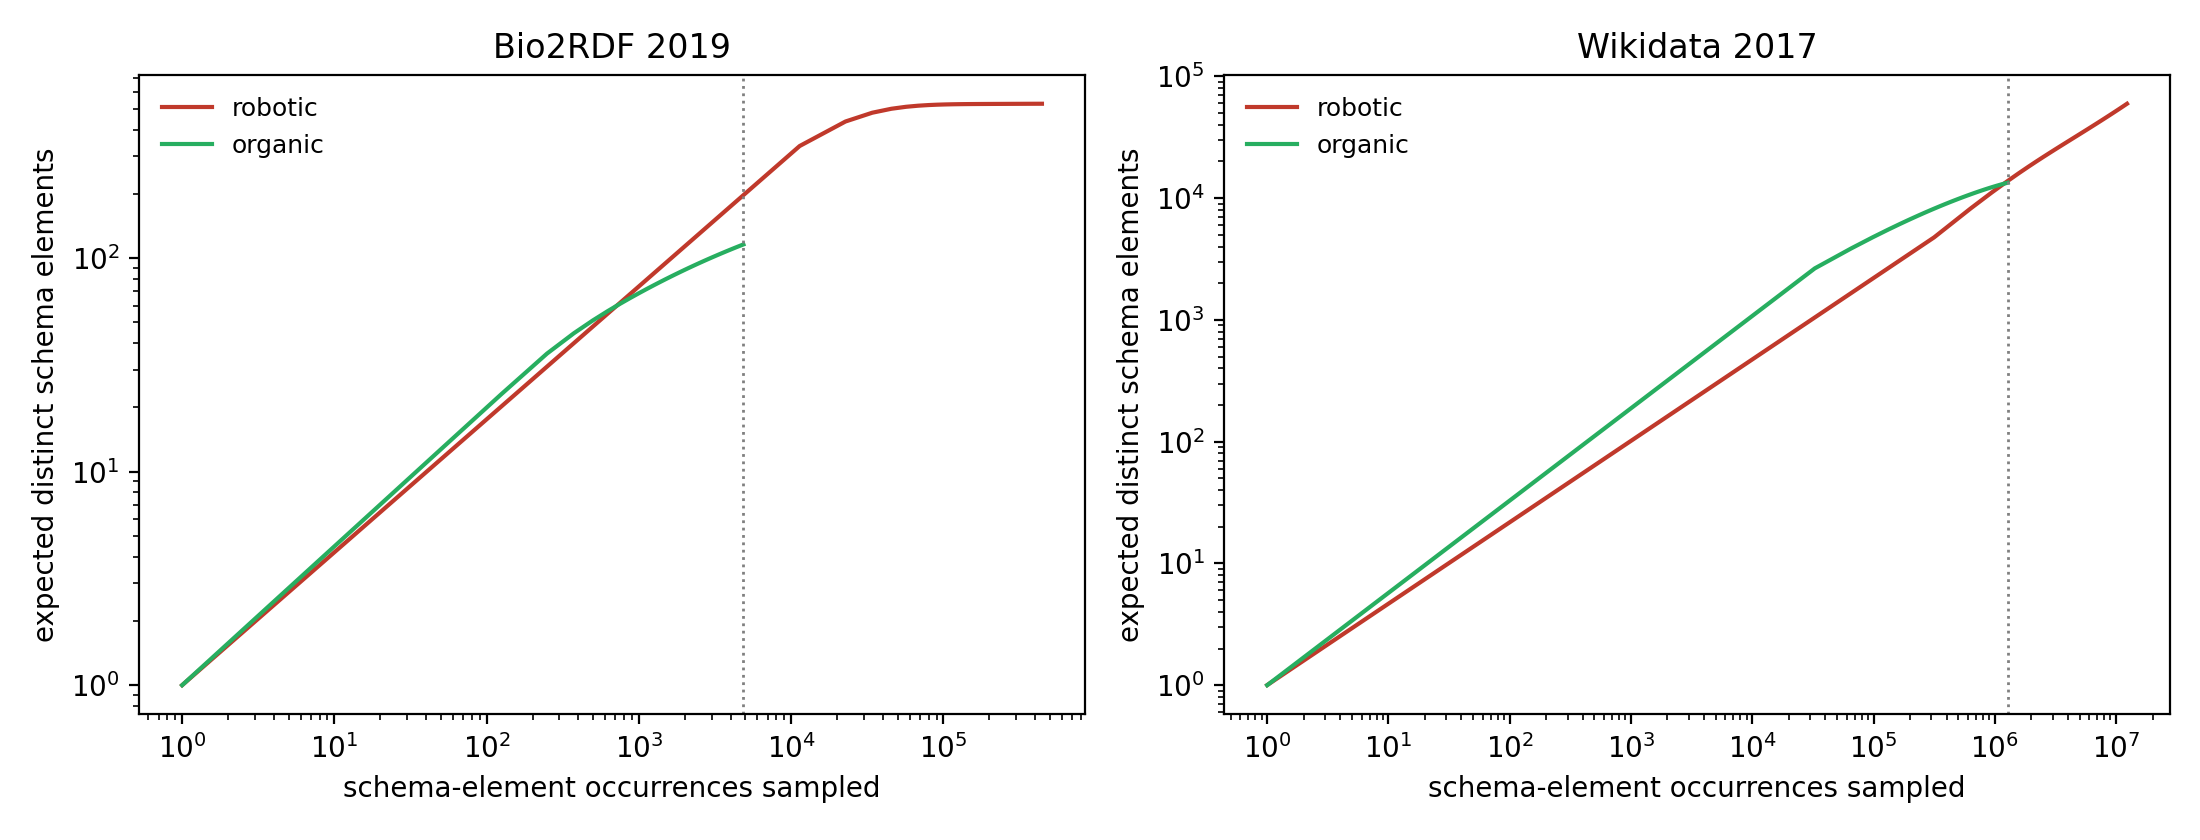
\includegraphics[width=0.95\textwidth]{rarefaction.png}
    \caption{Individual-based rarefaction curves (expected distinct schema elements vs.\ schema-element occurrences sampled, both axes log-scaled) for organic (green) and robotic (red) logs. The dotted line marks the organic log's sampling effort. For Bio2RDF the robotic curve rises well above organic at equal effort; for Wikidata the two curves are close, and organic is in fact richer per occurrence until effort equalizes.}
    \label{fig:rarefaction}
\end{figure}

\begin{table}[ht]
\centering
\caption{Schema coverage at equal sampling effort. Robotic logs are rarefied down to the number of schema-element occurrences observed in the corresponding organic log.}
\label{tab:rarefaction}
\begin{tabular}{l|r|r}
\hline
Comparison (equal effort) & Organic distinct elements (coverage) & Robotic distinct elements, rarefied (coverage) \\
\hline
Bio2RDF 2019 ($n=4{,}855$ occ.) & 116 (21.3\%) & $\approx$208 (38.2\%) \\
Wikidata 2017 ($n=1{,}279{,}731$ occ.) & 13,394 (12.8\%) & $\approx$13,846 (13.3\%) \\
\hline
\end{tabular}
\end{table}

The two KGs behave oppositely. For \textbf{Bio2RDF}, even at identical sampling effort the robotic log recovers roughly $1.8\times$ more distinct schema elements than the organic log (208 vs.\ 116; 38.2\% vs.\ 21.3\%), and its rarefaction curve saturates near the full schema. Robotic clients therefore genuinely exercise a broader part of this small, specialized schema, consistent with automated enumeration or dumping. For \textbf{Wikidata}, the picture reverses: at equal effort organic and robotic are nearly indistinguishable (13.3\% vs.\ 12.8\%), and at \emph{lower} effort organic queries are actually richer per occurrence (Figure~\ref{fig:rarefaction}, right). Here the large raw coverage gap in Table~\ref{tab:5} (57\% vs.\ 13\%) is almost entirely an artifact of robotic logs being two orders of magnitude larger, rather than evidence of broader robotic interest.

This size dependence is reinforced by how concentrated each log is on once-seen elements (Table~\ref{tab:singletons}). Two thirds of the schema elements counted for \emph{Wikidata-robotic-2017} are used exactly once; removing these singletons (the elements most exposed to one-off or erroneous uses) drops its coverage from 57.1\% to 18.9\% and shrinks the robotic-to-organic coverage ratio from $4.4\times$ to $2.0\times$. By contrast, \emph{Bio2RDF-robotic-2019} has a single singleton: its breadth is exercised repeatedly and is robust. In practical terms, robotic ``coverage'' on a very large KG such as Wikidata largely reflects query volume and a long tail of one-off references, whereas on a compact KG such as Bio2RDF it reflects systematic, repeated traversal of the schema.

\begin{table}[ht]
\centering
\caption{Singleton sensitivity. Schema elements used exactly once, and coverage with vs.\ without singletons (2017 logs for Wikidata, 2019 for Bio2RDF).}
\label{tab:singletons}
\begin{tabular}{l|r|r|r|r}
\hline
Log & Used elements & Singletons (\%) & Coverage & Coverage w/o singletons \\
\hline
Wikidata robotic & 59,603 & 39,900 (67\%) & 57.1\% & 18.9\% \\
Wikidata organic (full) & 13,394 & 3,412 (25\%) & 12.8\% & 9.6\% \\
Bio2RDF robotic & 529 & 1 (0.2\%) & 97.1\% & 96.9\% \\
Bio2RDF organic & 116 & 32 (28\%) & 21.3\% & 15.4\% \\
\hline
\end{tabular}
\end{table}

\subsection{Knowledge Graph Usage Patterns }
Thus far, we have introduced a method for calculating SPARQL schema coverage, which quantifies interactions with KGs through SPARQL queries. This measure may provide only a superficial view of KG usage. Knowing that a schema element was queried does not necessarily indicate its frequency of usage or temporal consistency. In this section, we present the results of the methods described in Section \ref{sec:s6}, focusing on the frequency distribution and temporal changes in KG usage. For this analysis, we have used unique queries.

\begin{figure}
    \centering
    
\includegraphics[width=0.9\textwidth]{image10.png} 
    \caption{Frequency distribution of schema elements across datasets (A–M). The datasets include: A) Bio2RDF All log2013\_kg2024, B) Bio2RDF All log2019\_kg2024,  C) Bio2RDF robotic log2019\_kg2024, D) Bio2RDF organic log2019\_kg2024, E) Wikidata organic log2017\_kg2017, F) Wikidata organic log2017\_kg2018,  G) Wikidata robotic log2017\_kg2017, H) Wikidata organic log2017\_kg2017, L) Wikidata robotic log2018\_kg2018, M) Wikidata organic log2018\_kg2018. The plot's color represents it's log type: blue for all logs, red for robotic logs, and green for organic logs. }
     \label{fig:l6}
\end{figure}

\subsubsection{Frequency Distribution of Schema Elements}
As described in Section \ref{sec:s61}, we analyze schema element usage patterns by visualizing the frequency distribution of elements across various intervals of robotic and organic query logs from Bio2RDF and Wikidata. Figure \ref{fig:l6} illustrates this distribution, where the y-axis represents the normalized monthly count of schema elements (logarithmic scale), while the x-axis represents the index assigned to each schema element. The Bio2RDF contain 545 schema elements, whereas Wikidata 2017 and 2018 include 104,314 and 98,462 elements, respectively. The color scheme distinguishes log types: green represents organic logs, red represents robotic logs, and blue represents all logs (organic and robotic combined). The plots (A–M) exhibit a consistent trend: a sharp decline in schema element usage frequency, suggesting that most schema elements are infrequently used.

Plot A (Bio2RDF All log2013\_kg2024) exhibits a more gradual decline in schema element usage compared to Plot B (Bio2RDF All log2019\_kg2024). Plot C (Bio2RDF robotic log2019\_kg2024) demonstrates a higher maximum frequency, with a log count approaching 4, whereas Plot D (Bio2RDF organic log2019\_kg2024) peaks at around 2. This contrast highlights the greater intensity of schema element usage in Bio2RDF robotic queries.

Plots E and F (Wikidata All organic log2017\_kg2017 and Wikidata All organic log2017\_kg2018) show a similar distribution of schema element usage across two different versions of Wikidata. Both intervals of robotic logs in Wikidata, Plot G and Plot L (Wikidata robotic log2017\_kg2017 and Wikidata robotic log2018\_kg2018), exhibit steep declines in schema element usage, with maximum frequencies exceeding a log count of 6.In contrast, Plot H (Wikidata organic log2017\_kg2017) and Plot M (Wikidata organic log2018\_kg2018) peak around 5, indicating less intensive schema element usage in organic queries.

Across all datasets, both organic and robotic queries display a sharp decline in schema element usage. However, robotic queries exhibit higher initial usage, with greater peak frequencies and broader schema element usage, followed by a steeper decline.

\paragraph{\textbf{Wilcoxon signed-rank test.}}We applied the Wilcoxon signed-rank test, as described in Section \ref{sec:s61}, to assess the consistency in schema element usage frequency between the two intervals of query logs for both Bio2RDF and Wikidata datasets.

For Bio2RDF, comparing Bio2RDF All log2013\_kg2024 with Bio2RDF All log2019\_kg2024 yielded a statistic of 6250.000 (p-value = 0.000), indicating a statistically significant difference in schema element usage between these intervals.

For Wikidata, the Wilcoxon signed‐rank test revealed significant changes in schema element usage frequency over time. Specifically, the comparison of the robotic logs (Wikidata robotic log2017\_kg2017 vs. Wikidata robotic log2018\_kg2018) yielded a test statistic of 126,884,288.500 (p-value = 0.000), while the organic logs (Wikidata organic log2017\_kg2017 vs. Wikidata organic log2018\_kg2018) produced a statistic of 607,273.000 (p-value = 0.000). These findings indicate that schema element usage in Wikidata varied significantly between the examined intervals.

\paragraph{\textbf{Changes in Used Schema Element Ranking}}
Using Equation \ref{eq:4}, introduced in Section \ref{sec:s61}, we computed Spearman's rank correlation and found weak to moderate consistency in schema element usage ranking across datasets. For the Bio2RDF logs (Bio2RDF All log2013\_kg2024 and Bio2RDF All log2019\_kg2024), the correlation coefficient of $\rho = 0.158$ ($p = 0.00497$) indicates a weak positive correlation. However, significant rank changes were observed for individual elements, such as \sloppy  % Allows words to break over lines more easily
\href{http://bio2rdf.org/kegg_vocabulary:Target}{kegg\_vocabulary:Target} (dropped 171 ranks), \href{http://bio2rdf.org/drugbank_vocabulary:group}{drugbank\_vocabulary:group} (dropped 167 ranks), and \href{http://bio2rdf.org/kegg_vocabulary:Disease}{kegg\_vocabulary:Disease} (dropped 165 ranks).

For the Wikidata robotic logs (Wikidata robotic log2017\_kg2017 vs. Wikidata robotic log2018\_kg2018), a correlation coefficient of $\rho = 0.484$ ($p = 0$) suggests a
moderate positive correlation, with notable rank changes for schema elements such as 
\href{http://www.wikidata.org/entity/Q4220917}{film award} (Q4220917) (fell by 458 ranks), 
\href{http://www.wikidata.org/entity/Q2831984}{comic book album} (Q2831984) (fell by 443 ranks), and 
\href{http://www.wikidata.org/entity/Q1667921}{novel series} (Q1667921) (fell by 437 ranks).

For the Wikidata organic logs (Wikidata organic log2017\_kg2017 vs. Wikidata organic log2018\_kg2018), a correlation coefficient ($\rho = 0.571$, $p = 7.46 \times 10^{-167}$) indicates a moderate positive correlation, with extreme rank changes for elements such as 
\href{http://www.wikidata.org/prop/direct/P1811}{P1811} (dropped 212 ranks), 
\href{http://www.wikidata.org/entity/Q811534}{remarkable tree} (Q811534) (rose 200 ranks), and 
\href{http://www.wikidata.org/prop/direct/P1423}{P1423} (dropped 182 ranks).

These rank shifts highlight changes in user interactions with the KG. The weak correlation ($\rho = 0.158$) observed for Bio2RDF may be partially attributed to the 6-year interval. In contrast, the Wikidata logs, which had a one-year interval, showed moderate positive correlations ($\rho = 0.484$ for robotic logs and $\rho = 0.571$ for organic logs). The stronger correlations for Wikidata suggest a more consistent use of schema elements over a shorter time frame.

% To evaluate consistency in the relative rank ordering of the schema element pairs between two intervals, we calculated the concordance index (C-index), as defined in Equation~\ref{eq:5}. 
% For the Bio2RDF logs, comparing the intervals of 2013 and 2019, the concordance index (C-index) was 0.539. This indicates a moderate level of agreement in the relative rank ordering of schema element pairs between these two years. For the Wikidata organic logs, comparing the intervals of 2017 and 2018, the concordance index (C-index) was 0.639, reflecting a slightly higher consistency in the rank ordering of schema elements between the two periods. These results suggest varying degrees of stability in the relative ranking of schema elements across the different datasets and time intervals.

\subsubsection{Frequent Schema Types}
As described in Section \ref{sec:s62}, we analyze the most frequently queried schema types to identify common elements that persist across different time intervals and log types. Figure \ref{fig:l8} illustrates the top 10 schema types queried across multiple datasets, comparing robotic and organic query logs from Wikidata and Bio2RDF. The x-axis represents the log-transformed total count of schema usages, while the y-axis lists the schema types. In this diagram, colors indicate log types: green for organic logs, red for robotic logs, and blue for all logs (both organic and robotic). Common schema classes across paired datasets are highlighted in bold.


Plot A and Plot B (Bio2RDF All log 2013 vs. 2019) show that four out of the ten schema types—\href{http://bio2rdf.org/omim:Gene}{omim:Gene}, \href{http://bio2rdf.org/wormbase:Gene}{wormbase:Gene}, \href{http://bio2rdf.org/drugbank:Target}{drugbank:Target}, and \href{http://bio2rdf.org/drugbank:Drug}{drugbank:Drug}—remain highly frequent despite a six-year gap between the two intervals. Plot C and Plot D (robotic vs. organic Bio2RDF queries of 2019) share only two common elements: \href{http://bio2rdf.org/drugbank:Drug}{drugbank:Drug} and \href{http://bio2rdf.org/phrmgkb:Variation}{phrmgkb:Variation}.

Plot E and Plot F (Wikidata All organic log 2017 with KG versions of 2017 and 2018) reveal a notable update in schema types, with \href{https://www.wikidata.org/wiki/Q142}{"France (Q142)"} newly classified as a schema type, while the rest of the frequently used schema types remain consistent with those from 2017. Plot G and Plot H (Wikidata robotic vs. organic 2017) share only three common elements: \href{https://www. wikidata.org/wiki/Q5}{"human (Q5)"}, \href{https://www.wikidata.org/wiki/Q11424}{"film (Q11424)"}, and \href{https://www.wikidata.org/wiki/Q515}{"city (Q515)"}. Plot L and Plot M (Wikidata robotic vs. organic 2018) also have three common elements: \href{https://www.wikidata.org/wiki/Q5}{"human (Q5)"}, \href{https://www.wikidata.org/wiki/Q11424}{"film (Q11424)"}, and \href{https://www.wikidata.org/wiki/Q21191270}{"television series episode (Q21191270)"}. Notably, \href{https://www.wikidata.org/wiki/Q5}{"human (Q5)"} and \href{https://www.wikidata.org/wiki/Q11424}{"film (Q11424)"} remain frequent across both 2017 and 2018 for both robotic and organic query types.

The comparison of the top 50 schema types across different intervals and query types further reveals that 24\% of the elements are common between Bio2rdf 2013 and 2019, 42\% overlap between robotic and organic queries in Bio2rdf 2019. For Wikidata, the overlap between robotic and organic queries is 30\% in 2017 and 36\% in 2018, with a 46\% commonality when comparing organic queries across the two years and 32\% common between robotic queries across 2017 and 2018.

Together, the analyses using both the top 10 and top 50 thresholds demonstrate that a core set of schema elements consistently drives query activity across these KGs. This consistency demonstrates the fundamental role of these schema types in shaping user interactions, regardless of temporal or query-type variations. In practical terms, this stable core is exactly the set that a documentation effort, an autocomplete feature, or a query-recommendation tool for the KG could prioritize with confidence.

\paragraph{\textbf{Content-level caveat: example-query contamination.}} Inspecting the top organic Wikidata elements reveals a confounding factor that any usage study should control for. The item \href{https://www.wikidata.org/wiki/Q6581072}{\emph{female} (Q6581072)} is recorded 9,331 times in \emph{Wikidata-organic-2017}, whereas its symmetric counterpart \href{https://www.wikidata.org/wiki/Q6581080}{\emph{male} (Q6581080)} does not appear at all. Such a perfect asymmetry between two otherwise interchangeable values is implausible for genuine end-user information needs; it is instead the signature of demonstration and example queries (the Wikidata Query Service example set queries \emph{female} but not \emph{male}) populating part of the ``organic'' log. This observation also illustrates the class-extraction caveat of Section~\ref{s3}.2: \emph{female} is counted here as a type because it is used as the object of \texttt{wdt:P31}/\texttt{wdt:P279} somewhere in the data, even though in queries it functions as a property value rather than a class. We therefore treat such elements with caution and discuss example-query contamination as a limitation in Section~\ref{s5}.

 \begin{figure}
    \centering
    
\includegraphics[width=0.8\textwidth]{image7.png} 
    \caption{The most frequent schema types across datasets (A–M). The datasets include: A) Bio2RDF All log2013\_kg2024, B) Bio2RDF All log2019\_kg2024,  C) Bio2RDF robotic log2019\_kg2024, D) Bio2RDF organic log2019\_kg2024, E) Wikidata organic log2017\_kg2017, F) Wikidata organic log2017\_kg2018,  G) Wikidata robotic log2017\_kg2017, H) Wikidata organic log2017\_kg2017, L) Wikidata robotic log2018\_kg2018, M) Wikidata organic log2018\_kg2018. The plot's color represents it's log type: blue for all logs, red for robotic logs, and green for organic logs. Bold labels indicate common schema classes that appear across paired datasets side by side.}
     \label{fig:l8}
\end{figure}

\paragraph{\textbf{Pairwise Schema Type Usage of Bio2RDF.}}

This analysis aims to investigate how pairwise schema type patterns that represent relationships between schema types from different Bio2RDF subgraphs have been used in queries over time. We examine the evolution of this type of federated querying by comparing Bio2RDF query logs from 2013 (log\_2013, covering 17 subgraphs) and 2019 (log\_2019, covering 26 subgraphs), as outlined in Section \ref{sec:s62}.

A pairwise pattern here is a query triple that links a type from one subgraph to a type from another via a (typically variable) predicate, i.e., an attempt to join data across datasets. The number of \emph{distinct} cross-subgraph join patterns observed in queries rose from \textbf{3 in log\_2013 to 22 in log\_2019} --- roughly a sevenfold increase in federated querying over time. We report this as a count rather than a fraction of ``possible'' patterns: the space of possible cross-subgraph joins is large (the schema exhibits 430 directed cross-subgraph type-to-type edges across 26 subgraphs) and, because observed joins use variable predicates rather than specific schema edges, a ``used-out-of-possible'' ratio would compare two different notions. The robust and reproducible quantity is the increase in distinct observed join patterns.

Figure \ref{fig:l7} presents a heatmap illustrating the pairwise schema type usage across Bio2RDF subgraphs for log\_2013 and log\_2019. The results highlight a significant increase in the diversity of dataset integration in 2019 relative to 2013. This shift reflects broader advancements in data accessibility and integration practices within the bioinformatics community. The observed increase is likely attributable to the adoption of a single query endpoint for all datasets in 2019, which improved accessibility compared to the multiple endpoints used in 2013.

\begin{figure}
    \centering
    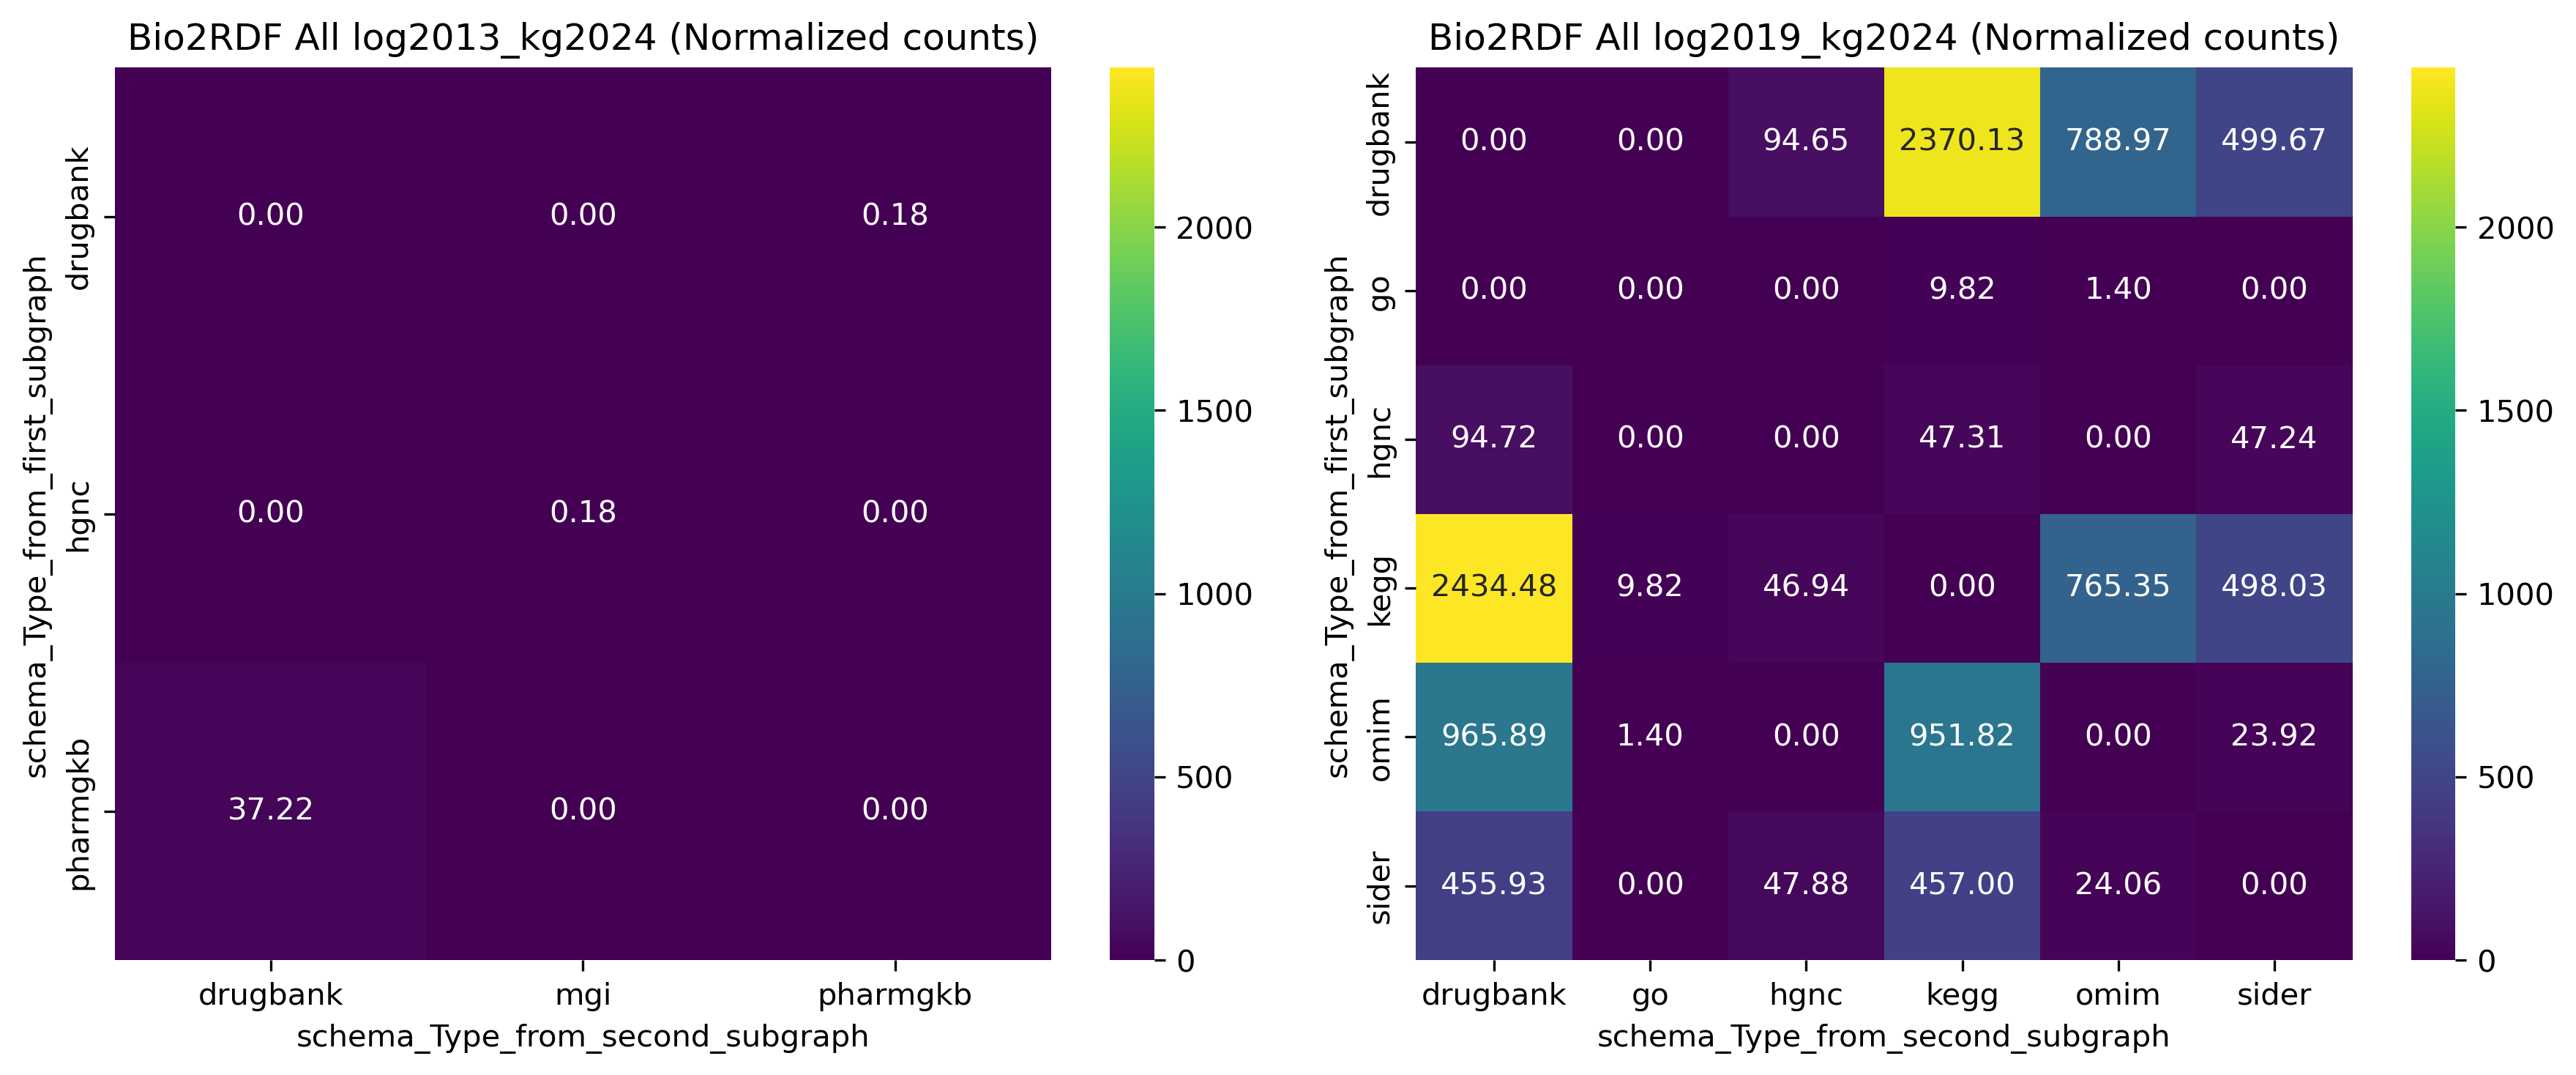
\includegraphics[width=0.8\textwidth]{image24.png} 
    \caption{Heatmap of the pairwise co-occurrence of schema types from two different subgraphs of log 2013 vs. 2019
}
     \label{fig:l7}
\end{figure}

Figure \ref{fig:l9} presents an overview of the usage metadata generated by the proposed method. This approach processes SPARQL queries and KGs to produce usage metadata. The extracted metadata includes SPARQL schema coverage, the schema elements used, their associated usage frequencies, and the generated schema for the respective KGs. The metadata for each dataset is available online for download\footnote{\url{https://github.com/MaastrichtU-IDS/KG_usage_metadata/tree/main/metadata-files}} in CSV and RDF formats.

\begin{figure}
    \centering
    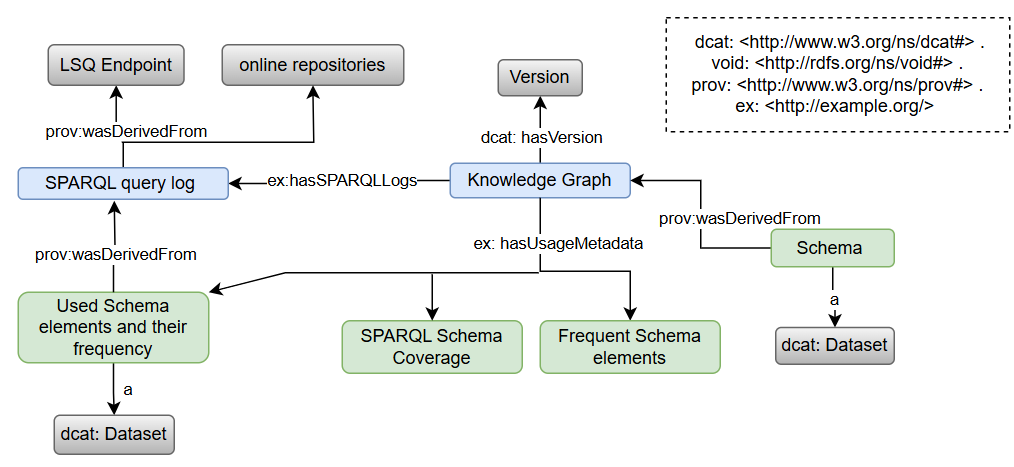
\includegraphics[width=0.8\textwidth]{image16.png} 
    \caption{Usage metadata model
}
    \label{fig:l9}
\end{figure}


\section{Discussion}\label{s5}
In this study, we analyzed SPARQL query logs to explore how users interact with knowledge graphs (KGs) by addressing two key questions: (1) How can we quantify the usage of a KG? and (2) Do frequency distribution and ranking analyses of used KG elements reveal usage patterns over different log intervals or across organic (human-driven) and robotic (bot-driven) query types? We applied the proposed method to the both robotic and organic query logs from Bio2RDF and Wikidata, uncovering several patterns in schema element usage.

To quantify the overall usage of a KG, we introduced the SPARQL schema coverage metric, which measures the proportion of schema elements that are explicitly referenced in queries. Raw coverage differs markedly between robotic and organic logs (robotic 97\% for Bio2RDF and 60\% for Wikidata; organic 21\% and 14\%), which might suggest that automated processes simply access a broader range of the schema. However, robotic and organic logs also differ in size by up to two orders of magnitude, so raw coverage conflates breadth of interest with sheer query volume. The size-controlled rarefaction analysis (Section~\ref{sec:rarefaction}) disentangles the two, and the conclusion is KG-dependent rather than a blanket statement about ``machine vs.\ human'' querying. For Bio2RDF, robotic logs cover roughly $1.8\times$ more of the schema than organic logs \emph{even at equal sampling effort}, so the broader robotic footprint there is a genuine behavioral difference (systematic, repeated traversal of a compact, specialized schema). For Wikidata, the gap essentially vanishes at equal effort, and organic queries are even richer per query at small samples; the large raw gap is mostly a volume artifact, amplified by a long tail of one-off references (two thirds of robotic Wikidata elements are used exactly once). The practical lesson is that schema coverage must be interpreted relative to sampling effort and to KG scale, and that ``robotic queries cover more'' holds for a small specialized KG but not for a very large one.

A further difference between the two query types is \emph{syntactic}, and it reinforces the organic/robotic distinction on an axis independent of schema breadth. In the Bio2RDF 2019 logs, robotic queries are almost entirely well-formed, standards-compliant SPARQL (about 99.5\% of unique robotic queries parse), whereas organic logs are far noisier: a large fraction of unique organic entries are not valid SPARQL at all but injected non-SPARQL text (e.g., blog-comment spam submitted to the public endpoint), and the genuinely non-standard queries that remain---using Virtuoso extensions such as \texttt{bif:contains} (full-text search), \texttt{OPTION}, and the \texttt{LIKE} operator---originate overwhelmingly from organic (human, web-form) traffic rather than from automated clients. In other words, the vendor-specific full-text and option syntax is a human behavior here, not a robotic one. This also cautions that ``valid query'' counts are sensitive to both log hygiene (non-SPARQL contamination of organic logs) and to engine-specific syntax; we verified that the validity rate itself is not an artifact of the chosen parser, since three independent SPARQL~1.1 parsers (a strict grammar, the parser used here, and a Rust engine) agree on validity for 98--99\% of queries.

Beyond coverage, we observed a pronounced long-tail distribution in the frequency of schema element usage in both datasets. While a few schema elements are queried very frequently, the vast majority are rarely used. This long-tail phenomenon is significant because it demonstrates that only a limited set of elements captures most of the user attention, despite the overall diversity in accessed elements. Although schema coverage and usage frequency analyses capture different dimensions of query behavior (i.e., the breadth of elements accessed versus the extent of their usage), they together provide a comprehensive view of usage patterns without implying a direct causal relation between them.

We computed Spearman’s rank correlations based on the frequency rankings of common schema elements in dataset pairs. Over a longer time span (e.g., Bio2RDF All logs: 2013 vs. 2019), the weak correlation suggests shifting rankings over time. In contrast, moderate correlation in shorter intervals of Wikidata robotic logs (2017 vs. 2018) and Wikidata organic logs (2017 vs. 2018), indicates greater consistency in the near term.

Focusing on the most frequently queried schema types, our findings reveal a dual pattern in both the top 10 and top 50 elements. In the top 10 analysis, a small stable core, typically comprising 2 to 4 elements, appears consistently across different datasets, time intervals, and query types, while the remaining elements tend to vary. In the top 50 frequent elements, we observe an overlap of 24\% to 46\% common elements across different comparisons. This indicates that although a core set of schema elements remains persistently frequent (likely due to their fundamental role or inherent relevance), the majority of frequently queried elements are variable, reflecting evolving user interests or updates in data structures. Importantly, the persistent core can be leveraged in KG documentation and design, ensuring that these key elements are prioritized and optimized to better serve user needs.

% Taken together, these findings provide a nuanced view of KG usage patterns. Both organic and robotic queries exhibit a long-tail distribution in schema element usage; however, robotic queries access a broader range of elements, while organic queries concentrate on a smaller subset. Recognizing this distinction is important because it reveals that, despite similar overall distributions, the type of query (automated vs. human-driven) influences the breadth of schema elements used. Furthermore, the presence of a stable core in the top 10—coupled with substantial variability in the remaining elements—and the Spearman’s rank correlation results highlight a dual pattern of stability and evolution in KG usage. Short-term consistency exists among the most frequently queried elements, while longer time spans witness more substantial reordering in element popularity. These insights offer valuable perspectives for optimizing knowledge graph design and query strategies to better cater to diverse user needs.

In addition, the pairwise schema type co-occurrence analysis in Bio2RDF reveals that the number of distinct cross-subgraph join patterns observed in queries increased from 3 in the 2013 logs to 22 in the 2019 logs. This substantial increase in federated querying indicates an enhanced emphasis on integrating multiple datasets over time, likely driven by improved accessibility, such as the shift from multiple query endpoints in 2013 to a unified endpoint in 2019. These results demonstrate the importance of designing KGs that support robust federated query capabilities, especially in data-driven fields like bioinformatics.

In conclusion, the findings offer a detailed understanding of KG usage patterns and present valuable guidance for refining KG design and query strategies to better address user needs.

This study has several limitations, which also point to future work.

\emph{Comparability of the two KGs.} The log collection periods differ (Bio2RDF $\sim$30 months vs.\ Wikidata $\sim$9 months) and the schemas differ in scale by roughly two orders of magnitude. We mitigate the first with time-normalized counts and the second by reporting coverage primarily within each KG and by the size-controlled rarefaction analysis; nonetheless, cross-KG coverage percentages should not be read as a direct ranking. Direct comparison over equal-length time windows and across KGs of similar scale remains valuable future work.

\emph{What counts as a class in Wikidata.} Our type set for Wikidata is a data-driven operationalization (objects of \texttt{wdt:P31}/\texttt{wdt:P279}); defining a ``class'' in Wikidata is genuinely contested \cite{brasileiro2016applying,piscopo2018who,patelschneider2024class}. This operationalization is heterogeneous: it mixes heavily instantiated classes with class-like individuals that have few or no instances, and using only \texttt{wdt:P279} (whose subproperties we do not follow) under-counts class-like elements. Because the Wikidata type set is so large and partly under-instantiated, the low Wikidata coverage is partly definitional rather than purely behavioral. The singleton-sensitivity analysis (Table~\ref{tab:singletons}) bounds the influence of one-off, possibly erroneous uses, but a principled, instance-aware notion of ``class'' for usage studies is an open problem.

\emph{Explicit reference vs.\ effective usage.} We count a schema element as used when it is explicitly written in a query. This is the right notion for documentation, interface, and deprecation decisions, but it does not capture the subclasses and subproperties that a property path (e.g.\ \texttt{wdt:P31/wdt:P279*}) traverses at evaluation time and that also contribute to answers. A closure-based notion of effective usage, which would attribute usage to every element that contributes answers, is a natural and substantial extension.

\emph{Example-query contamination and weighting.} As the \emph{female}/\emph{male} asymmetry illustrates, ``organic'' logs can be contaminated by demonstration and example queries, which inflate the apparent usage of the elements those examples reference. Identifying and down-weighting example-driven traffic, and complementing our deduplicated (intent-diversity) counts with volume-weighted counts, would sharpen the behavioral interpretation.

% Another avenue for further exploration lies in addressing the semantic gap between user queries and KG content. To investigate how well current KGs align with user needs, identifying potential mismatches and opportunities to adjust KG schema to improve responsiveness to real-world queries. This could involve developing metrics to quantify the alignment between user intent and KG schema.


\section{Conclusion}\label{s6}
This study introduces a novel approach for analyzing SPARQL query logs to gain deeper insights into user interactions with knowledge graphs (KGs). To identify usage patterns, we introduce the SPARQL schema coverage metric and conduct frequency distribution and ranking analyses of queried KG elements across different log intervals and both organic and robotic query types from Bio2RDF and Wikidata.
The findings reveal that both query types in both datasets exhibit a long-tail distribution in schema element usage. Raw coverage is higher for robotic queries (60--97\%) than organic ones (14--21\%), but a size-controlled (rarefaction) analysis shows that this gap reflects a genuine behavioral difference only for the compact Bio2RDF schema; for the much larger Wikidata it is largely a consequence of robotic logs being far larger.
Furthermore, the temporal analysis of frequently queried elements identifies a stable core of elements that consistently drive user queries over time. Additionally, Spearman’s rank correlation of common elements across Wikidata intervals demonstrates relatively stable rankings over short-term periods (one year). However, in Bio2RDF, longer time spans (six years) exhibit greater changes in the ranking of used elements.
To improve cross-KG comparisons, future research might involve analyzing standardized log collection periods and comparing datasets of similar scale. Overall, our findings advance the understanding of KG usage patterns and provide guidance for optimizing KG design, documentation, and query strategies, ultimately contributing to the development of more responsive and user-centric knowledge graphs.

The implementation of this method is publicly available on the GitHub repository: \url{https://github.com/MaastrichtU-IDS/KG_usage_metadata}.
\section{Acknowledgment}\label{s7}
This project has received funding from the European Union’s Horizon 2020 research and innovation program under the Marie Skłodowska-Curie grant agreement No 860801.

%\subsection{}\label{s1.1}

%\begin{figure}[t]
%\includegraphics{}
%\caption{Figure caption.}\label{f1}
%\end{figure}

%\begin{table*}
%\caption{} \label{t1}
%\begin{tabular}{lll}
%\hline
%&&\\
%&&\\
%\hline
%\end{tabular}
%\end{table*}

%%%%%%%%%%% The bibliography starts:

%%%%%%%%%%%%%%%%%%%%%%%%%%%%%%%%%%%%%%%%%%%%%%%%%%%%%%%%%%%%%
%%                  The Bibliography                       %%
%%                                                         %%
%%  ios1.bst will be used to                               %%
%%  create a .BBL file for submission.                     %%
%%                                                         %%
%%                                                         %%
%%  Note that the displayed Bibliography will not          %%
%%  necessarily be rendered by Latex exactly as specified  %%
%%  in the online Instructions for Authors.                %%
%%                                                         %%
%%%%%%%%%%%%%%%%%%%%%%%%%%%%%%%%%%%%%%%%%%%%%%%%%%%%%%%%%%%%%


\nocite{*}
% if your bibliography is in bibtex format, use those commands:
\bibliographystyle{ios1}           % Style BST file.
\bibliography{bibliography}        % Bibliography file (usually '*.bib')

% or include bibliography directly:
%\begin{thebibliography}{0}
%\bibitem{r1} F. Author, Information about cited object.
%
%\bibitem{r2} S. Author and T. Author, Information about cited object.
%\end{thebibliography}
% \begin{thebibliography}{0}

% \bibitem{1} B. Abu-Salih, \textit{Domain-specific knowledge graphs: A survey}, \textit{Journal of Network and Computer Applications} \textbf{185} (2021), 103076.

% \bibitem{2} W. Ali, M. Saleem, B. Yao, A. Hogan, and A.-C. Ngonga Ngomo, \textit{A survey of RDF stores \& SPARQL engines for querying knowledge graphs}, \textit{The VLDB Journal} (2022), 1-26.

% \bibitem{3} L. Asprino and M. Ceriani, \textit{How is Your Knowledge Graph Used: Content-Centric Analysis of SPARQL Query Logs}, in: \textit{International Semantic Web Conference}, Springer Nature Switzerland, 2023, pp. 197-215.

% \bibitem{4} A. Bielefeldt, J. Gonsior, and M. Krötzsch, \textit{Practical Linked Data Access via SPARQL: The Case of Wikidata}, in: \textit{LDOW@WWW}, 2018.

% \bibitem{5} A. Bonifati, W. Martens, and T. Timm, \textit{An analytical study of large SPARQL query logs}, \textit{The VLDB Journal} \textbf{29}(2) (2020), 655-679.

% \bibitem{6} C. Buil-Aranda, M. Ugarte, M. Arenas, and M. Dumontier, \textit{A preliminary investigation into SPARQL query complexity and federation in Bio2RDF}, in: \textit{Alberto Mendelzon International Workshop on Foundations of Data Management}, 2015, p. 196.

% \bibitem{7} M. Saleem, M. I. Ali, A. Hogan, Q. Mehmood, and A.-C. Ngonga Ngomo, \textit{LSQ: the linked SPARQL queries dataset}, in: \textit{The Semantic Web-ISWC 2015: 14th International Semantic Web Conference}, Springer International Publishing, 2015, pp. 261-269.

% \bibitem{8} C. Stadler, M. Saleem, Q. Mehmood, C. Buil-Aranda, M. Dumontier, A. Hogan, and A.-C. Ngonga Ngomo, \textit{LSQ 2.0: A linked dataset of SPARQL query logs}, \textit{Semantic Web Preprint} (2024), 1-23.

% \bibitem{9} \url{https://www.npmjs.com/package/sparqljs}.

% \bibitem{10} F. Belleau, M.-A. Nolin, N. Tourigny, P. Rigault, and J. Morissette, \textit{Bio2RDF: towards a mashup to build bioinformatics knowledge systems}, \textit{Journal of Biomedical Informatics} \textbf{41}(5) (2008), 706-716.

% \bibitem{11} A. Hogan, E. Blomqvist, M. Cochez, C. d’Amato, G. De Melo, C. Gutierrez, S. Kirrane, et al., \textit{Knowledge graphs}, \textit{ACM Computing Surveys (Csur)} \textbf{54}(4) (2021), 1-37.

% \bibitem{12} M. Mohammadi, \textit{(Semi-) Automatic Construction of Knowledge Graph Metadata}, in: \textit{European Semantic Web Conference}, Springer International Publishing, 2022, pp. 171-178.

% \bibitem{14} M. Mohammadi, and M. Dumontier,\textit{ Analyzing SPARQL Query Logs: A Study on Schema Coverage and Query Content}, \textit{Semantic Web Applications and Tools for Health Care and Life Sciences (SWAT4HCLS)}, 2024, \url{https://ceur-ws.org/Vol-3890/paper-14.pdf}.

% \bibitem{15} K. Möller, M. Hausenblas, R. Cyganiak, S. Handschuh, and G.A. Grimnes, \textit{Learning from Linked Open Data Usage: Patterns \& Metrics}, in: \textit{Proc. Web Science Conf. (WebSci’10)}, 2010.

% \bibitem{16} A. Bonifati, W. Martens, and T. Timm, \textit{An Analytical Study of Large SPARQL Query Logs}, \textit{Proceedings of the VLDB Endowment} \textbf{11}(2017), 149–161, Issue 2.

% \bibitem{17} M. Kaminski and E.V. Kostylev, \textit{Complexity and Expressive Power of Weakly Well-Designed SPARQL}, \textit{Theory of Computing Systems} (2018), 1–38, \url{https://doi.org/10.1007/s00224-017-9802-9}.

% \bibitem{18} F. Picalausa and S. Vansummeren, \textit{What are real SPARQL queries like?}, in: \textit{Proc. Int.Workshop on SemanticWeb Information Management (SWIM’11)}, ACM, 2011, pp. 6.

% \bibitem{19} J. Lorey and F. Naumann, \textit{Detecting SPARQL Query Templates for Data Prefetching}, in: \textit{Proc. 10th Extended Semantic Web Conference (ESWC’13)}, Springer, 2013, pp. 124–139.

% \bibitem{20} A. Raghuveer, \textit{Characterizing Machine Agent Behavior through SPARQL Query Mining}, in: \textit{Proc. 2nd Int. Workshop on Usage Analysis and the Web of Data (USEWOD’12)}, 2012.

% \bibitem{21} L. Rietveld and R. Hoekstra, \textit{Man vs. Machine: Differences in SPARQL Queries}, in: \textit{Proc. 4th USEWOD Workshop on Usage Analysis and the Web of Data}, 2014.

% \bibitem{22} C. Peng, F. Xia, M. Naseriparsa, and F. Osborne, \textit{Knowledge graphs: Opportunities and challenges}, \textit{Artificial Intelligence Review} \textbf{56}(11) (2023), 13071-13102.

% \bibitem{23} C. Spearman, \textit{The proof and measurement of association between two things}, (1961).

% \bibitem{24} S. Malyshev, M. Krötzsch, L. González, J. Gonsior, and A. Bielefeldt, \textit{Getting the most out of Wikidata: Semantic technology usage in Wikipedia’s knowledge graph}, in: \textit{The Semantic Web–ISWC 2018: 17th International Semantic Web Conference}, Springer International Publishing, 2018, pp. 376-394.


% \end{thebibliography}


\end{document}

